\documentclass[../src/handouts/main.tex]{subfiles}
% note that the CWD (.) above is the output directory of pdflatex
% (<repo-root-dir>/build)

% path that contains required images
\graphicspath{ {../src/handouts/figures/} }

% This document depends on the other sections, which provide the
% following references (in the order of references in this section):
%   enum:con-tree-state
%   prop:con-connected-vertex
%   thm:con-cut-edge-cycle
%   def:con-component
%   def:con-path-cycle
%   def:con-complete
%   def:con-loop
%   def:intro-set-operations
%   eq:intro-pascal
%   def:intro-set-shorthand
%   def:con-degree
%   def:intro-bijection
%   subsec:con-graph-isomorphism
% As a result, compiling only this document gives undefined references.

% prevent \recall theorems outside this section
% if this section is compiled solely
\def\sectionprefix{tree}%

\begin{document}

% TODO: use TikZ to replace almost all figures

\section{Trees and Distance}

This section is the chapter 2 in the textbook "Introduction to Graph Theory".

\supp{Tree and its techniques (breadth first search, depth first search) are common in programming contest, computer aided design (CAD), software verification, logic analysis, etc. As a result, this section is important in this course.}



\subsection{Basic Properties}



\subsubsection{Properties of Trees}

\begin{definition}{}{tree-tree}
  A graph with no cycle is \textbf{acyclic}.

  A \textbf{forest} is an acyclic graph.

  A \textbf{tree} is a connected acyclic graph.

  A \textbf{leaf} (pendant vertex, terminal) is a vertex of degree 1.

  A \textbf{spanning subgraph} of $G$ is a subgraph with vertex set $V(G)$.

  A \textbf{spanning tree} is a spanning subgraph that is a tree.
\end{definition}

\begin{figure}[htbp]
  % TODO: TikZ version
  \centering
  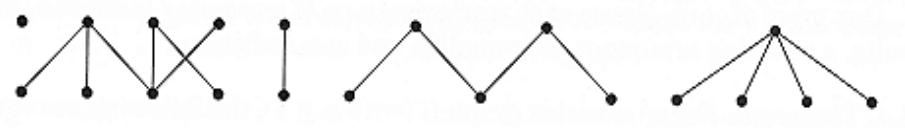
\includegraphics[width=.6\textwidth]{tree-tree-introduction}
  \caption{Examples of forests and trees.}
\end{figure}

\begin{lemma}{}{tree-deleting-leaf}
  (2.1.3. Lemma in text)
  Every tree with at least two vertices has at least two leaves.
  Deleting a leaf from an $n$-vertex tree produces a tree with $n-1$ vertices.
\end{lemma}

A graph with only two vertices and an edge is also a tree by definition, so such a graph is covered by \cref{lem:tree-deleting-leaf}.

\textbf{Proof} of \cref{lem:tree-deleting-leaf}:
\begin{enumerate*}
  \item \supp{In this proof, it is better to have at least 3 nodes in a tree. However, in the textbook it used a tree with 2 vertices as an example.}
  \item In a tree (connected acyclic graph) with at least 3 nodes, an endpoint of a maximal nontrivial path has no neighbor other than its neighbor on the path. Hence the endpoints of a such a path are leaves.
  \item Let $v$ be a leave of a tree $G$ of three nodes, and let $G' = G - v$.
  \item A vertex of degree 1 (vertex $v$) belongs to no path connecting two other vertices. Therefore, for $u, w \in V\left( G' \right)$, every $u,w$-path in $G$ is also in $G'$. Hence $G'$ is connected. Since deleting a vertex cannot create a cycle, $G'$ is also acyclic. Thus $G'$ is a tree with $n - 1$ vertices.
\end{enumerate*}

\begin{figure}[htbp]
  % TODO: TikZ version
  \centering
  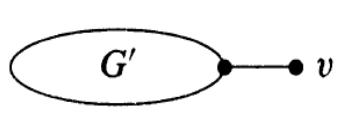
\includegraphics[width=.3\textwidth]{tree-deleting-leaf}
  \caption{An illustration of deleting a leaf $v$ from $G$ to form $G'$.}
  \label{fig:tree-deleting-leaf}
\end{figure}

\begin{theorem}{}{tree-tree-stat}
  (2.1.4. Theorem in text; introduced in \cpageref{enum:con-tree-state} previously)

  For an $n$-vertex graph $G$ (with $n \geq 1$ ), the following statements are equivalent (and characterize the trees with $n$ vertices).
  \begin{enumerate*}
    \item $G$ is connected and has no cycles.
    \item $G$ is connected and has $n - 1$ edges.
    \item $G$ has $n - 1$ edges and no cycles.
    \item For $u, v \in V(G)$, $G$ has exactly one $u,v$-path.
  \end{enumerate*}
\end{theorem}

Traditionally, to prove \cref{thm:tree-tree-stat}, we need to prove these 4 statements pairwisely (6 iff. pairs). Nonetheless, in this proof, we prove any two of the statements \{ connected, acyclic, $n - 1$ edges\} for a graph imply the other one, and prove the statement 4 is equivalent to any of the three statements, saying statement 1 (connected and acyclic), with 4 iff. pairs in total instead of 6.

Note that your assumption must be correct before any proof. For example, these 4 statements must be correct before proofs. Under wrong assumptions, you have only wrong results.

\textbf{Proof} of statement 1 (connected, acyclic) implying statements 2 and 3 ($n - 1$ edges) in \cref{thm:tree-tree-stat}:

\begin{enumerate*}
  \vspace{-.25em} % magic number to make these enumerated list look alike
  \item We use induction on $n$, which is the number of vertices in the graph $G$.
  \item For $n = 1$, an acyclic 1-vertex graph has no edge.
  \item For $n > 1$:
    \vspace{.5em}
    \begin{enumerate*}
      \item We suppose that the implication holds for graphs with fewer than $n$ vertices.
      \item Given an acyclic connected graph $G$, \cref{lem:tree-deleting-leaf} provides a leaf $v$ and states that $G' = G - v$ also is acyclic and connected (see figure above).
      \item Applying the induction hypothesis to $G'$ yields $e \left( G' \right) = n - 2$. Since only one edge is incident to $v$, we have $e(G) = e \left( G' \right) + 1 = n - 1$.
    \end{enumerate*}
    \vspace{.25em} % more space after enumerate*
\end{enumerate*}
\vspace{.5em} % more space after enumerate*

\textbf{Proof} of statement 2 (connected, $n - 1$ edges) implying statements 1 and 3 (acyclic) in \cref{thm:tree-tree-stat}:
\begin{enumerate*}
  \item We use proof by contradiction.
  \item Suppose the graph $G$ has a cycle.
  \item Delete edges from cycles of $G$ one by one to form $G'$ until the resulting graph $G'$ is acyclic. \supp{We cannot delete edges that are not parts of some cycles, or we will make the graph disconnected (no path from a component to the other one).}
  \item Recall \cref{prop:con-connected-vertex}: The minimum number of edges in a connected graph with $n$ vertices is $n - 1$.
  \item To have $G'$ connected, $e\left( G' \right) = n - 1$.
  \item Since we are given $e(G) = n - 1$, no edges were deleted. Thus $G' = G$, and $G$ is acyclic.
\end{enumerate*}
\vspace{.5em} % more space after enumerate*

\textbf{Proof} of statement 3 ($n - 1$ edges, acyclic) implying statements 1 and 2 (connected) in \cref{thm:tree-tree-stat}:
\begin{enumerate*}
  \item We use proof by contradiction with some calculation.
  \item Let $G_1,\, \ldots,\, G_k$ be the components of $G$. If $k \geq 2$, then $G$ is disconnected.
  \item Since every vertex appears in a single component, $\sum_i n \left( G_i \right) = n$. Since $G$ has no cycles, $e \left( G_i \right) = n \left( G_i \right) - 1$ for each $i$.
  \item Summing over $i$ yields $e(G) = \sum _i \left( n \left( G_i \right) - 1 \right) = n - k$.
  \item We are given $e(G) = n - 1$, so $k = 1$, and $G$ is connected.
\end{enumerate*}
\vspace{.5em} % more space after enumerate*

\textbf{Proof} of statement 1 (connected, acyclic) implying statement 4 (unique $u,v$-path) in \cref{thm:tree-tree-stat}:
\begin{enumerate*}
  \item We use proof by contradiction.
  \item Since the graph $G$ is connected, each pair of vertices is connected by a path. \supp{We cannot say that these is no path to violate the assumption of a conencted graph.}
  \item If some pair ov vertices $u,\, v$ is connected by \textbf{more than one path}, a cycle is formed by any two of the paths as illustrated in \cref{fig:tree-tree-stat}. It contradicts to the assumption of an acyclic graph.
  \item As a result, there is only a single path between any two vertices in $G$.
\end{enumerate*}
\vspace{.5em} % more space after enumerate*

\clearpage % magic escape to prevent paragraph overlapping with the footer
\textbf{Proof} of statement 4 (unique $u,v$-path) implying statement 1 (connected, acyclic):
\begin{enumerate*}
  \item We use direct method and proof by contradiction.
  \item If there is a $u,v$-path for every $u,\, v \in V(G)$, then $G$ is connected.
  \item If $G$ has a cycle $C$, then $G$ has two $u,v$-paths for $u,\, v \in V(C)$. It contradicts to the assumption that there is only a single path between $u$ and $v$.
  \item Hence, $G$ is acyclic (this also forbids loops).
\end{enumerate*}
\vspace{.5em} % more space after enumerate*

\begin{figure}[htbp]
  % TODO: TikZ version
  \centering
  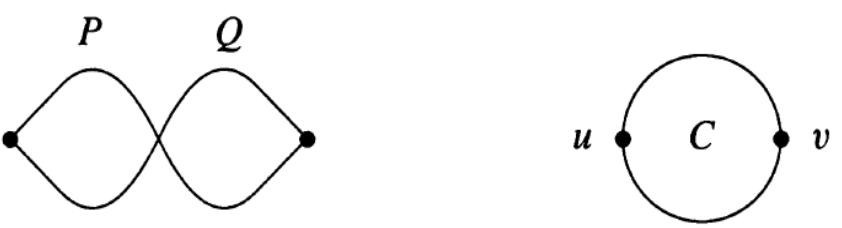
\includegraphics[width=.5\textwidth]{tree-tree-stat}
  \caption{A graph to illustrate the proof of equivalence between statements 1 and 4 in \cref{thm:tree-tree-stat}.}
  \label{fig:tree-tree-stat}
\end{figure}

\begin{corollary}{}{tree-cut-edge}
  (2.1.5. Corollary in text)
  \begin{enumerate*}
    \item Every edge of a tree is a cut-edge.
    \item Adding one edge to a tree forms exactly one cycle.
    \item Every connected graph contains a spanning tree.
  \end{enumerate*}
\end{corollary}

\textbf{Proof} of \cref{cor:tree-cut-edge}:
\begin{enumerate*}
  \item A tree has no cycles, so \cref{thm:con-cut-edge-cycle} implies that every edge is a cut-edge.
  \item A tree has a unique path linking each pair of vertices (\cref{thm:tree-tree-stat} statement 4), so joining two vertices by an edge creates exactly one cycle.
  \item As in the proof of statement 2 implying 1 and 3 in \cref{thm:tree-tree-stat}, iteratively deleting edges from cycles in a connected graph yields a connected acyclic subgraph, which is a spanning tree.
\end{enumerate*}

\begin{proposition}{}{tree-spanning-tree-edge-a}
  (2.1.6. Proposition in text)
  If $T,\, T'$ are spanning trees of a connected graph $G$ and $e \in E(T) - E \left( T' \right)$, then there is an edge $e' \in E \left( T' \right) - E(T)$ such that $\underline{T - e + e'}$ is a spanning tree of $G$.
\end{proposition}

\textbf{Proof} of \cref{prop:tree-spanning-tree-edge-a}:
\begin{enumerate*}
  \item By \cref{cor:tree-cut-edge} statement 1, every edge of $T$ is a cut-edge of $T$. Let $U$ and $U'$ be the two components of $T - e$.
  \item Since $T'$ is connected, $T'$ has an edge $e'$ with endpoints in $U$ and $U'$.
  \item Now $T - e + e'$ is connected, has $n(G) - 1$ edges, and is a spanning tree of $G$. Since the new edge $e'$ is not in either component, it doesn't form a cycle.
  \item (In \cref{fig:tree-spanning-tree-edge}, $T$ is bold, $T'$ is solid, and they share two edges.)
\end{enumerate*}

\begin{figure}[htbp]
  % TODO: TikZ version
  \centering
  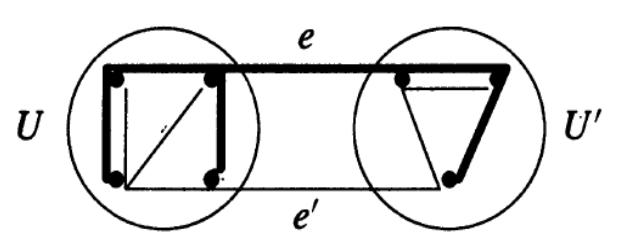
\includegraphics[width=.4\textwidth]{tree-spanning-tree-edge}
  \caption{An example for a cut-edge in spanning tree $T$ (bold edges) and $T'$ (solid edges).}
  \label{fig:tree-spanning-tree-edge}
\end{figure}

\begin{proposition}{}{tree-spanning-tree-edge-b}
  (2.1.7. Proposition in text)
  If $T,\, T'$ are spanning trees of a connected graph $G$ and $e \in E(T) - E \left( T' \right)$, then there is an edge $e' \in E \left( T' \right) - E(T)$ such that $\underline{T + e - e'}$ is a spanning tree of $G$.
\end{proposition}

\textbf{Proof} of \cref{prop:tree-spanning-tree-edge-b}:
\begin{enumerate*}
  \item \supp{In graph theory (Geometry), addition and subtraction do not have the same meaning in Algebra. In Algebra, $a - b + c = a + c - b$.}
  \item By \cref{cor:tree-cut-edge} statement 2, the graph $T' + e$ contains a unique cycle $C$.
  \item Since $T$ is acyclic, there is an edge $e' \in E(C) - E(T)$ (the edge in the cycle $C$ but not in the spanning tree $T$).
  \item Deleting $e'$ breaks the only cycle in $T' + e$. Now $T' + e - e'$ is connected and acyclic and is a spanning tree of $G$.
  \item (In the figure above, adding $e$ to $T$ creates a cycle $C$ of length five; all four edges of $C - e$ belong to $E(T) - E \left( T' \right)$ and can serve as $e'$.)
\end{enumerate*}



\subsubsection{Distance in Trees and Graphs}

\begin{definition}{}{tree-distance}
  The \textbf{distance} from $u$ to $v$, written $d_G(u,\, v)$, is the \textbf{least} length of a $\bm{u, v}$\textbf{-path}.

  The \textbf{diameter} of a graph $G$, written $\diam G$, is defined by $\max _{u,\, v \in V(G)} d(u,\, v)$. That is, the maximum distance among all pairs of vertices in $V(G)$.

  The \textbf{eccentricity} of a vertex $u$, written $\epsilon(u)$, is $\max _{v \in V(G)} d(u, v)$. That is, the maximum distance from the vertex $u$ to the other vertices.

  The \textbf{radius} of a graph $G$, written $\rad G$, is $\min _{u \in V(G)} \epsilon(u)$.
\end{definition}

Note that the diameter and radius of a graph do not have the same meanings for a circle. So, the diameter of a graph doesn't necessary the same as half of its radius.

The eccentricity of a trivial component (a graph with only a vertex; \cref{def:con-component}) is 0.

See \cref{fig:tree-distance} for an example of attributes in \cref{def:tree-distance}.

\begin{figure}[htbp]
  \centering
  \def\nd{2.5cm}% node distance
  \newcommand{\shiftTL}{(30:\nd * 1)}% shift for the top-left triangle
  \newcommand{\shiftBM}{(30:\nd * 2)}% shift for thee bottom-middle triangle
  \newcommand{\shiftRR}{(30:\nd * 3)}% shift for the right rectangle
  \begin{tikzpicture}[
      every node/.style = {draw, circle, inner sep=.1cm},
      thickness/.style = {ultra thick}
    ]

    % left triangle
    \node (a1) at (0, 0) {4}; % bottom
    \node (a2) at (30:\nd) {3}; % right
    \node (a3) at (90:\nd) {4}; % top

    % top-left triangle
    % multiplying 1.064 to align nodes with the right rectangle
    % sin(30 degree) / sin(110 degree) * 2 = 1.064
    % reference: law of sines
    % see he bottom-middle triangle for better understanding
    \node (b1) at ([shift=\shiftTL] +110:\nd * 1.064) {4};
    \node (b2) at ([shift=\shiftTL] +70:\nd * 1.064) {4};

    % bottom-middle triangle
    % multiplying 1.064 to align nodes with the left triangle
    % multiplying 0.940 to align c3 with c2 and c4
    % sin(30 degree) / sin(110 degree) * 2 = 1.064
    % sin(70 degree) = 0.940
    \node (c1) at ([shift=\shiftBM] 0:0) {2};
    \node (c2) at ([shift=\shiftBM] -110:\nd * 1.064) {3};
    \node (c3) at ([shift=\shiftBM] -90:\nd * 1.064 * 0.940) {4};
    \node (c4) at ([shift=\shiftBM] -70:\nd * 1.064) {3};

    % right rectangle
    % multiplying 1.414 to align d3 with d2 and d4
    % sec(45 degree) = 1.414
    \node (d1) at ([shift=\shiftRR] 0:0) {4};
    \node (d2) at ([shift=\shiftRR] 0:\nd) {4};
    \node (d3) at ([shift=\shiftRR] -45:\nd * 1.414) {4};
    \node (d4) at ([shift=\shiftRR] -90:\nd) {3};

    % edges not belonging to the longest path
    \draw[thickness] (a3) -- (a2) -- (b1) -- (b2) -- (a2);
    \draw[thickness] (c1) -- (c2) -- (c3) -- (c4) -- (c1);
    \draw[thickness] (d1) -- (d3) -- (d4) -- (d2);

    % longest path
    \draw[thickness, red] (a3) -- (a1) -- (a2) --
    (c1) --
    (d4) -- (d1) -- (d2) -- (d3);
  \end{tikzpicture}
  \caption{In this graph, each vertex is labeled with its eccentricity $\epsilon(u)$. The radius is 2, the diameter is 4, and the length of the longest path (in red) is 7. Recall \cref{def:con-path-cycle}: A path contains distinct vertices.}
  \label{fig:tree-distance}
\end{figure}

\begin{supplement}
  In \cref{fig:tree-distance}, we introduced the diameter of a graph. To connect devices in a local area network (LAN), with quite few switches, the locations of switches limits the locations of devices that requires Ethernet. With too many switches, the cost is not acceptable. As a result, we need to take a balance between the diameter and the cost in a network.

  Speaking of the distance in \cref{def:tree-distance}, on a social media, there may be a mutual friend between persons $A$ and $B$. In such a case, the distance between $A$ and $B$ is 2 (degree 1). In a social network (in real world, not online), the distance between any two strangers is at most 7 (at most 6 people between; at most degree 6). With social media, the distance may be down to 4 (degree 3). See \textit{six degrees of separation}\footnote{Wikipedia contributors. (2024, April 16). Six degrees of separation. In Wikipedia, The Free Encyclopedia. Retrieved 03:00, April 17, 2024, UTC, from \url{https://en.wikipedia.org/w/index.php?title=Six_degrees_of_separation&oldid=1219175664}} for more information.

  Paul Erdős (1913--1996) is one of the most prolific mathematicians in the 20th century because it published around 1,500 mathematical papers.

  Since Erdős is popular, mathematicians defined \textbf{Erdős number} as follows. The Erdős number of Erdős is 0; the Erdős number of the coauthors with Erdős is 1; the Erdős number of the coauthors with the coauthors with Erdős is 2, etc.
\end{supplement}

\begin{theorem}{}{tree-diameter}
  (2.1.11. Theorem in text)
  If $G$ is a simple graph, then $\diam G \geq 3$ implies $\diam \bar{G} \leq 3$.
\end{theorem}

\textbf{Proof} of \cref{thm:tree-diameter}:
\begin{enumerate}
  \item (When $\diam G = 1$, $G$ is a complete graph (\cref{def:con-complete}).)
  \item (When $\diam G = 2$, in $G$, every pair of vertex either is adjacent or has a common neighbor.)
  \item When $\diam G > 2$, there exist nonadjacent vertices $u, v \in V(G)$ ($u \nleftrightarrow v$; \cref{def:con-loop}) with no common neighbor. Such $u$ and $v$ in $\bar{G}$ must either be adjacent or have a common neighbor.
  \item Hence in $G$, every $x \in V(G) - \{u, v\}$ (vertices other than $u$ and $v$; \cref{def:intro-set-operations}) is nonadjacent to either $u$ or $v$, or both. This makes $x$ adjacent to either $u$ or $v$, or both in $\bar{G}$.
    \begin{supplement}
      \item Cases for the relation between a vertex $x$ to $u$ and $v$ in $\bar{G}$ to derive the relation in $G$:
      \begin{enumerate}
        \item $x \leftrightarrow u$ but $x \nleftrightarrow v$ in $\bar{G}$, as vertices in the left set (circle) in \cref{fig:tree-diameter}. As a result, $x \nleftrightarrow u$ but $x \leftrightarrow v$ in $G$.
        \item $x \nleftrightarrow u$ and $x \nleftrightarrow v$ in $\bar{G}$, for $x$ in the middle set in \cref{fig:tree-diameter}. Thus, $x \leftrightarrow u$ and $x \leftrightarrow v$ in $G$.
        \item $x \nleftrightarrow u$ but $x \leftrightarrow v$ in $\bar{G}$, for $x$ in the right set in \cref{fig:tree-diameter}. Thus, $x \leftrightarrow u$ but $x \nleftrightarrow v$ in $G$.
      \end{enumerate}
    \end{supplement}
  \item Since also $u v \in E(\bar{G})$, for every pair $x, y$ there is an $x, y$-path of length at most 3 in $\bar{G}$ through $\{u, v\}$.
  \item Hence diam $\bar{G} \leq 3$.
\end{enumerate}

\begin{figure}[htbp]
  % TODO: TikZ version
  \centering
  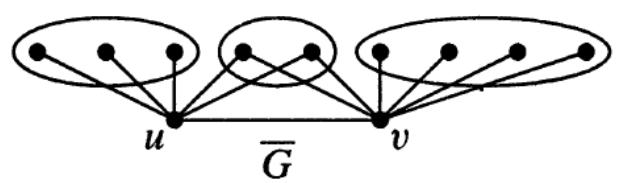
\includegraphics[width=.5\textwidth]{tree-diameter}
  \caption{An illustration for the proof of \cref{thm:tree-diameter}. In the three sets for $\bar{G}$, from left to right, these sets include vertices adjacent to only $u$, to both $u$ and $v$, and to only $v$, respectively.}
  \label{fig:tree-diameter}
\end{figure}

\begin{definition}{}{tree-center}
  (2.1.12. Definition in text)
  The \textbf{center} of a graph $G$ is the subgraph induced by the vertices of minimum eccentricity.
\end{definition}

Continuing from \cref{def:tree-center}, it means for some vertices in $V(G)$ with the globally minimum eccentricity (distance to their own farthest vertices), these vertices form the center of $G$.

\begin{theorem}{}{tree-center}
  (2.1.13. Theorem in text; Jordan [1869])
  The center of a tree is a vertex or an edge.
\end{theorem}

\textbf{Proof} of \cref{thm:tree-center}:
\begin{enumerate}
  \item We use induction on the number of vertices in a tree $T$, denoted by $n(T)$.

  \item Basis step: $n(T) \leq 2$ (1 or 2). With at most two vertices, the center is the entire tree.

  \item Induction step: $n(T) > 2$.
    \begin{enumerate}
      \item Form $T'$ by deleting every leaf of $T$. By \cref{lem:tree-deleting-leaf}, $T'$ is a tree.
      \item Since the internal vertices on paths between leaves of $T$ remain, $T'$ has at least one vertex.
      \item Every vertex at maximum distance in $T$ from a vertex $u \in V(T)$ is a leaf (otherwise, the path reaching it from $u$ can be extended farther).
      \item Since all the leaves have been removed and no path between two other vertices uses a leaf, $\epsilon_{T'}(u) = \epsilon_T(u) - 1$ for every $u \in V \left( T' \right)$.
      \item Also, the eccentricity of a leaf in $T$ is greater than the eccentricity of its neighbor in $T$. Hence the vertices minimizing $\epsilon_T(u)$ are the same as the vertices minimizing $\epsilon_{T'}(u)$.
      \item We have shown that $T$ and $T'$ have the same center.
      \item By the induction hypothesis, the center of $T'$ is a vertex or an edge.
    \end{enumerate}
\end{enumerate}

\begin{figure}[htbp]
  % TODO: TikZ version
  \centering
  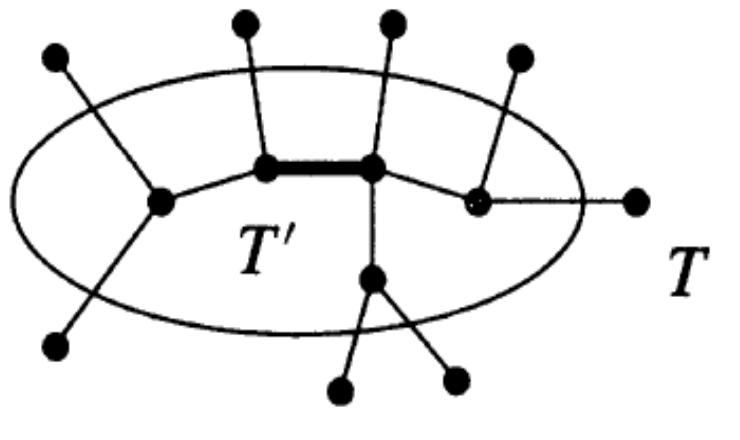
\includegraphics[width=.5\textwidth]{tree-center}
  \caption{An illustration for the proof of \cref{thm:tree-center}. $T$ is the original tree, while $T'$ is $T$ without its leaves.}
  \label{fig:tree-center}
\end{figure}

\begin{theorem}{}{tree-wiener}
  (2.1.14. Theorem in text)
  Among trees with $n$ vertices, the Wiener index of $G$ is $D(G)=\sum_{u, v \in V(G)} d_G(u, v)$. Under a fixed number of vertices in a graph, the Wiener index is minimized by a star and maximized by a path, both uniquely.
\end{theorem}

In \cref{thm:tree-wiener}, the Wiener index means the summation of distances for all pair of vertices. A star is a graph with a vertex in the center, and all the other vertices only adjacent to the center vertex. In other words, a star of $n + 1$ vertices is a complete bipartite graph $K_{1, n}$ (\cref{def:con-complete}).

\textbf{Proof} of \cref{thm:tree-wiener}:
\begin{enumerate}
  \item Our discussion focus on a connected graph with at least 1 vertices.
  \item For minimization:
    \begin{enumerate}
      \item Since a tree has $n - 1$ edges, it has $n - 1$ pairs of vertices at distance 1, and all other pairs have distance at least 2.  The star achieves this and hence minimizes $D(T)$.
      \item To show that no other tree achieves this, consider a leaf $x$ in $T$, and let $v$ be its neighbor. If all other vertices have distance 2 from $x$, then they must be neighbors of $v$, and $T$ is the star. The value is $D K _{1, n - 1} = (n - 1) + 2 \C{n - 1}{2} = (n - 1)^2$.
    \end{enumerate}

  \item For the maximization,
    \begin{enumerate}
      \item Consider first $D(P_n)$. This equals the sum of the distances from an endpoint $u$ to the other vertices, plus $D(P_{n - 1})$.

      \item We have $\sum_{v \in V(P_n)} d(u, v) = \sum_{i = 0}^{n - 1} i = \C{n}{2}$.

      \item Thus $D(P_n) = D(P_{n - 1}) + \C{n}{2}$.

      \item With Pascal's Formula (\cref{eq:intro-pascal}), $\C{n}{k} + \C{n}{k - 1} = \C{n + 1}{k}$, induction yields $D(P_n) = \C{n + 1}{3}$.

      \item We prove \textbf{by induction} on $n$ that among $n$-vertex tree, $P_n$ is the only tree that maximizes $D(T)$.

      \item Basis step: $n = 1$. The only tree with one vertex is $P_1$.

      \item Induction step: $n > 1$:
        \begin{enumerate}
          \item Let $u$ be a leaf of an $n$-vertex tree $T$.
          \item Now $D(T) = D(T - u) + \sum_{v \in V(T)} d(u, v)$.
          \item By the induction hypothesis, $D(T - u) \leq D(P_{n - 1})$, with equality if and only if $T - u$ is a path.
          \item Thus it suffices to show that $\sum_{v \in V(T)} d(u, v)$ is maximized only when $T$ is a path and $u$ is an endpoint of $T$.
          \item Consider the list of distances from $u$. In $P_n$, this list is $1,\, 2,\, \ldots,\, n - 1$, all distinct. A shortest path from $u$ to a vertex farthest from $u$ contains vertices at all distances from $u$, so in any tree the set of distances from $u$ to other vertices has no gaps.
          \item Thus any repetition makes $\sum_{v \in V(T)} d(u, v)$ smaller than when $u$ is a leaf of a path.
          \item When $T$ is not a path, such a repetition occurs.
        \end{enumerate}
    \end{enumerate}
\end{enumerate}

\begin{lemma}{}{con-subgraph-degree}
  (2.1.15. Lemma in text)
  If $H$ is a subgraph of $G$, then $d_G(u, v) \leq d_H(u, v)$.
\end{lemma}

\textbf{Proof} of \cref{lem:con-subgraph-degree}: Every $u, v$-path in $H$ appears also in $G$, so the shortest $u, v$-path in $G$ is no longer than the shortest $u, v$-path in $H$. For example, to go to the EE building from the Kuang-Fu student dormitory No.1, with the Dasyue road under maintenance, you need to take the other road with farther distance to the EE building.

\begin{corollary}{}{con-connected-wiener}
  (2.1.16. Corollary in text)
  If $G$ is a connected $n$-vertex graph, then $D(G) \leq D\left(P_n\right)$.
\end{corollary}

\textbf{Proof} of \cref{cor:con-connected-wiener}: Let $T$ be a spanning tree of $G$. By \cref{lem:con-subgraph-degree}, $D(G) \leq D(T)$. By \cref{thm:tree-wiener}, $D(T) \leq D\left(P_n\right)$.


\subsection{Spanning Trees and Enumeration}

Without considering graph isomorphism and different subtrees, with 3 vertices, there are 3 possible trees as the enumeration of 3 vertices.

\begin{figure}[htbp]
  \centering
  \begin{subfigure}[t]{.15\textwidth}
    \centering
    \tikz \node[draw, circle, fill=blue!25!white, inner sep=.1cm] {A};
    \caption{One vertex.}
    \label{fig:tree-enum-one}
  \end{subfigure}
  \begin{subfigure}[t]{.2\textwidth}
    \centering
    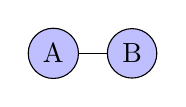
\begin{tikzpicture}[
        every node/.style = {draw, circle, fill=blue!25!white, inner sep=.1cm}
      ]
      \node (a) at (0, 0) {A}
      node (b) at (1, 0) {B};
      \draw (a) --(b);
    \end{tikzpicture}
    \caption{Two vertices.}
    \label{fig:tree-enum-two}
  \end{subfigure}
  \begin{subfigure}[t]{.4\textwidth}
    \centering
    \newcommand{\enumthree}[4]{%
      \node      (#1) at (#1 * 2 + 0.5, 1.75) {#1}%
      node[main] (#2) at (#1 * 2 + 0  , 0   ) {#2}%
      node[main] (#3) at (#1 * 2 + 0.5, 1   ) {#3}%
      node[main] (#4) at (#1 * 2 + 1  , 0   ) {#4};%
      \draw (#2) -- (#3) -- (#4)%
    }
    \begin{tikzpicture}[
        main/.style = {draw, circle, fill=blue!25!white, inner sep=.1cm}
      ]
      \enumthree{1}{B}{A}{C};
      \enumthree{2}{A}{B}{C};
      \enumthree{3}{A}{C}{B};
    \end{tikzpicture}
    \caption{Three vertices.}
    \label{fig:tree-enum-three}
  \end{subfigure}
  \caption{Enumeration of spanning trees.}
  \label{fig:tree-enum}
\end{figure}

To add a unique number (ID or code) to each tree in the enumeration for a given number of vertices, we need \cref{alg:tree-prufer-code}.

\begin{algorithm}{Prüfer code}{tree-prufer-code}
  (2.2.1. Algorithm.)
  Production of $f(T) = \left( a_1,\, \ldots,\, a_{n - 2} \right)$ for a tree with $n$ vertices.

  \textbf{Input}: A tree $T$ with vertex set $S \subseteq \N$.

  \textbf{Iteration}: At the $i$-th step, delete the least remaining leaf, and let $a_i$ be the \textit{neighbor} (parent) of this leaf.
\end{algorithm}

In exams, you may be asked to (1) answer the Prüfer code of a given tree, or (2) derive the tree for a given Prüfer code. You don't need to write down the pseudo-code of the Prüfer code algorithm.

See \cref{fig:tree-prufer-code} for an example of \cref{alg:tree-prufer-code}.

\begin{figure}[htbp]
  \centering
  \begin{subfigure}[t]{.3\textwidth} % step 0
    \centering
    \begin{tikzpicture}[
        every node/.style = {draw, circle, inner sep=.1cm},
        thickness/.style = {ultra thick},
        node distance = 0.5cm,
      ]
      \node (a1) {2};
      \node (b1) [right = of a1] {7} node (b2) [below = of b1] {6};
      \node (c1) [right = of b1] {1} node (c2) [below = of c1] {8};
      \node (d1) [right = of c1] {4} node (d2) [below = of d1] {5};
      \node (e1) [right = of d1] {3};
      \draw[thickness] (a1) -- (b1) -- (b2);
      \draw[thickness] (b1) -- (c1) -- (c2);
      \draw[thickness] (c1) -- (d1) -- (d2);
      \draw[thickness] (d1) -- (e1);
    \end{tikzpicture}
    \caption{Step 0: The original tree with vertex set $[7]$ (\cref{def:intro-set-shorthand}).}
    \label{fig:tree-prufer-code-0}
  \end{subfigure}

  \vspace{1em}

  \begin{subfigure}[t]{.3\textwidth} % step 1: delete 2
    \centering
    \begin{tikzpicture}[
        every node/.style = {draw, circle, inner sep=.1cm},
        thickness/.style = {ultra thick},
        node distance = 0.5cm,
      ]
      \node (b1) [right = of a1] {7} node (b2) [below = of b1] {6};
      \node (c1) [right = of b1] {1} node (c2) [below = of c1] {8};
      \node (d1) [right = of c1] {4} node (d2) [below = of d1] {5};
      \node (e1) [right = of d1] {3};
      \draw[thickness] (b1) -- (b2);
      \draw[thickness] (b1) -- (c1) -- (c2);
      \draw[thickness] (c1) -- (d1) -- (d2);
      \draw[thickness] (d1) -- (e1);
    \end{tikzpicture}
    \caption{Step 1: Delete 2, which has the least index among leaves. $a_1 = 7$, which is the parent of 2.}
    \label{fig:tree-prufer-code-1}
  \end{subfigure}
  \begin{subfigure}[t]{.3\textwidth} % step 2: delete 3
    \centering
    \begin{tikzpicture}[
        every node/.style = {draw, circle, inner sep=.1cm},
        thickness/.style = {ultra thick},
        node distance = 0.5cm,
      ]
      \node (b1) [right = of a1] {7} node (b2) [below = of b1] {6};
      \node (c1) [right = of b1] {1} node (c2) [below = of c1] {8};
      \node (d1) [right = of c1] {4} node (d2) [below = of d1] {5};
      \draw[thickness] (b1) -- (b2);
      \draw[thickness] (b1) -- (c1) -- (c2);
      \draw[thickness] (c1) -- (d1) -- (d2);
    \end{tikzpicture}
    \caption{Step 2: Delete 3. $a_2 = 4$.}
    \label{fig:tree-prufer-code-2}
  \end{subfigure}
  \begin{subfigure}[t]{.3\textwidth} % step 3: delete 5
    \centering
    \begin{tikzpicture}[
        every node/.style = {draw, circle, inner sep=.1cm},
        thickness/.style = {ultra thick},
        node distance = 0.5cm,
      ]
      \node (b1) [right = of a1] {7} node (b2) [below = of b1] {6};
      \node (c1) [right = of b1] {1} node (c2) [below = of c1] {8};
      \node (d1) [right = of c1] {4};
      \draw[thickness] (b1) -- (b2);
      \draw[thickness] (b1) -- (c1) -- (c2);
      \draw[thickness] (c1) -- (d1);
    \end{tikzpicture}
    \caption{Step 3: Delete 5. $a_3 = 4$.}
    \label{fig:tree-prufer-code-3}
  \end{subfigure}

  \vspace{1em}

  \begin{subfigure}[t]{.3\textwidth} % step 4: delete 4
    \centering
    \begin{tikzpicture}[
        every node/.style = {draw, circle, inner sep=.1cm},
        thickness/.style = {ultra thick},
        node distance = 0.5cm,
      ]
      \node (b1) [right = of a1] {7} node (b2) [below = of b1] {6};
      \node (c1) [right = of b1] {1} node (c2) [below = of c1] {8};
      \draw[thickness] (b1) -- (b2);
      \draw[thickness] (b1) -- (c1) -- (c2);
    \end{tikzpicture}
    \caption{Step 4: Delete 4. $a_4 = 1$.}
    \label{fig:tree-prufer-code-4}
  \end{subfigure}
  \begin{subfigure}[t]{.3\textwidth} % step 5: delete 6
    \centering
    \begin{tikzpicture}[
        every node/.style = {draw, circle, inner sep=.1cm},
        thickness/.style = {ultra thick},
        node distance = 0.5cm,
      ]
      \node (b1) [right = of a1] {7};
      \node (c1) [right = of b1] {1} node (c2) [below = of c1] {8};
      \draw[thickness] (b1) -- (c1) -- (c2);
    \end{tikzpicture}
    \caption{Step 5: Delete 6. $a_5 = 7$.}
    \label{fig:tree-prufer-code-5}
  \end{subfigure}
  \begin{subfigure}[t]{.3\textwidth} % step 6: delete 7
    \centering
    \begin{tikzpicture}[
        every node/.style = {draw, circle, inner sep=.1cm},
        thickness/.style = {ultra thick},
        node distance = 0.5cm,
      ]
      \node (c1) [right = of b1] {1} node (c2) [below = of c1] {8};
      \draw[thickness] (c1) -- (c2);
    \end{tikzpicture}
    \caption{Step 6: Delete 7. $a_6 = 1$.}
    \label{fig:tree-prufer-code-6}
  \end{subfigure}

  \caption{An example of \cref{alg:tree-prufer-code} (Prüfer code).}
  \label{fig:tree-prufer-code}
\end{figure}

\begin{example}[breakable]{}{tree-prufer-code}
  \def\nd{1cm}% node distance

  \textbf{Question}: Given Prüfer code 744171, what is the tree?

  By the induction hypothesis, there exists exactly one tree $T'$ having vertex set $S'$ and Prüfer code $a'$. Since every tree with Prüfer code $a$ is formed by adding the edge $x a_1$ to such a tree, there is at most one solution to $f(T) = a$. Furthermore, adding $x a_1$ to $T'$ does create a tree with vertex set $S$ and Prüfer code $a$, so there is at least one solution.

  \textbf{Answer}: Since there is 6 values in the given Prüfer code, there are 8 ($ = 6 + 2$) nodes in the tree. List vertices with indices in $[8]$ (\cref{def:intro-set-shorthand}) as follows.

  \begin{center}
    \begin{tikzpicture}[
        every node/.style = {draw, circle, inner sep=.1cm}
      ]
      \node foreach \i in {1, ..., 8} (\i) at (\nd * \i, 0) {\i};
    \end{tikzpicture}
  \end{center}

  Step 1: Vertices 2, 3, 5, 6, 8 are not in the Prüfer code, so they are leaves. Since the least vertex is deleted, and its parent is the first number in Prüfer code, we know that when vertex 2 is deleted, its parent is 7. Draw the edge 72, and let the leaves in red text. Vertices without color may be leaves in future steps.

  \begin{center}
    \begin{tikzpicture}[
        every node/.style = {draw, circle, inner sep=.1cm},
        leaf/.style = {text=red},
        every edge/.style = {draw, ultra thick},
      ]
      \node foreach \i in {1, 3, 4, ..., 8} (\i) at (\nd * \i, 0) {\i};
      \node[leaf] (2) at (\nd * 2, 0) {2};
      \draw (7) edge[bend right=45, looseness=0.5] (2);
    \end{tikzpicture}
  \end{center}

  Step 2: The Prüfer code is now (44171). Vertices in $[8] - \{2\}$ but not in the Prüfer code are 3, 5, 6, 8. The least vertex is 3, and the first value in the Prüfer code is 4. Draw the edge 43.

  \begin{center}
    \begin{tikzpicture}[
        every node/.style = {draw, circle, inner sep=.1cm},
        leaf/.style = {text=red},
        every edge/.style = {draw, ultra thick},
      ]
      \node foreach \i in {1, 4, 5, ..., 8} (\i) at (\nd * \i, 0) {\i};
      \foreach \i in {2, 3} \node[leaf] (\i) at (\nd * \i, 0) {\i};
      \draw (7) edge[bend right=45, looseness=0.5] (2);
      \draw (4) edge (3);
    \end{tikzpicture}
  \end{center}

  Step 3: The Prüfer code is now (4171). Vertices in $[8] - \{2,\, 3\}$ but not in the Prüfer code are 5, 6, 8. The least vertex is 5, and the first value in the Prüfer code is 4. Draw the edge 54.

  \begin{center}
    \begin{tikzpicture}[
        every node/.style = {draw, circle, inner sep=.1cm},
        leaf/.style = {text=red},
        every edge/.style = {draw, ultra thick},
      ]
      \node foreach \i in {1, 4, 6, 7, 8} (\i) at (\nd * \i, 0) {\i};
      \foreach \i in {2, 3, 5} \node[leaf] (\i) at (\nd * \i, 0) {\i};
      \draw (7) edge[bend right=45, looseness=0.5] (2);
      \draw (4) edge (3);
      \draw (5) edge (4);
    \end{tikzpicture}
  \end{center}

  Step 4: The Prüfer code is now (171). Vertices in $[8] - \{2,\, 3,\, 5\}$ but not in the Prüfer code are 4, 6, 8. The least vertex is 4, and the first value in the Prüfer code is 1. Draw the edge 41.

  \begin{center}
    \begin{tikzpicture}[
        every node/.style = {draw, circle, inner sep=.1cm},
        leaf/.style = {text=red},
        every edge/.style = {draw, ultra thick},
      ]
      \node foreach \i in {1, 6, 7, 8} (\i) at (\nd * \i, 0) {\i};
      \foreach \i in {2, ..., 5} \node[leaf] (\i) at (\nd * \i, 0) {\i};
      \draw (7) edge[bend right=45, looseness=0.5] (2);
      \draw (4) edge (3);
      \draw (5) edge (4);
      \draw (1) edge[bend right=45, looseness=0.5] (4);
    \end{tikzpicture}
  \end{center}

  Step 5: The Prüfer code is now (71). Vertices in $[8] - \{2,\, 3,\, 4,\, 5\}$ but not in the Prüfer code are 6, 8. The least vertex is 6, and the first value in the Prüfer code is 7. Draw the edge 76.

  \begin{center}
    \begin{tikzpicture}[
        every node/.style = {draw, circle, inner sep=.1cm},
        leaf/.style = {text=red},
        every edge/.style = {draw, ultra thick},
      ]
      \node foreach \i in {1, 7, 8} (\i) at (\nd * \i, 0) {\i};
      \foreach \i in {2, ..., 6} \node[leaf] (\i) at (\nd * \i, 0) {\i};
      \draw (7) edge[bend right=45, looseness=0.5] (2);
      \draw (4) edge (3);
      \draw (5) edge (4);
      \draw (1) edge[bend right=45, looseness=0.5] (4);
      \draw (7) edge (6);
    \end{tikzpicture}
  \end{center}

  Step 6: The Prüfer code is now (1). Vertices in $[8] - \{2,\, 3,\, 4,\, 5,\, 6\}$ but not in the Prüfer code are 7, 8. The least vertex is 7, and the first value in the Prüfer code is 1. Draw the edge 17.

  \begin{center}
    \begin{tikzpicture}[
        every node/.style = {draw, circle, inner sep=.1cm},
        leaf/.style = {text=red},
        every edge/.style = {draw, ultra thick},
      ]
      \node foreach \i in {1, 8} (\i) at (\nd * \i, 0) {\i};
      \foreach \i in {2, ..., 7} \node[leaf] (\i) at (\nd * \i, 0) {\i};
      \draw (7) edge[bend right=45, looseness=0.5] (2);
      \draw (4) edge (3);
      \draw (5) edge (4);
      \draw (1) edge[bend right=45, looseness=0.5] (4);
      \draw (7) edge (6);
      \draw (1) edge[bend left=60, looseness=0.5] (7);
    \end{tikzpicture}
  \end{center}

  Step 7: Since a tree is connected, draw the edge 18 in the end.

  \begin{center}
    \begin{tikzpicture}[
        every node/.style = {draw, circle, inner sep=.1cm},
        leaf/.style = {text=red},
        every edge/.style = {draw, ultra thick},
      ]
      \foreach \i in {1, ..., 8} \node[leaf] (\i) at (\nd * \i, 0) {\i};
      \draw (7) edge[bend right=45, looseness=0.5] (2);
      \draw (4) edge (3);
      \draw (5) edge (4);
      \draw (1) edge[bend right=45, looseness=0.5] (4);
      \draw (7) edge (6);
      \draw (1) edge[bend left=60, looseness=0.5] (7);
      \draw (1) edge[bend right=60, looseness=0.5] (8);
    \end{tikzpicture}
  \end{center}
\end{example}

\begin{theorem}{Cayley's Formula [1889]}{tree-cayley}
  (2.2.3. Theorem in text)
  For a set $S \subseteq \N$ of size $n$, there are $n^{n - 2}$ trees with vertex set $S$.
\end{theorem}

\textbf{Proof} of \cref{thm:tree-cayley} (Prüfer [1918]):
\begin{enumerate}
  \item This holds for $n = 1$, so we assume $n \geq 2$.
  \item We prove that \cref{alg:tree-prufer-code} defines a bijection $f$ from the set of trees with vertex set $S$ to the set $S^{n - 2}$ of lists of length $n - 2$ from $S$.
  \item We must show for each $a = \left(a_1,\, \ldots,\, a_{n - 2}\right) \in S^{n - 2}$ that exactly one tree $T$ with vertex set $S$ satisfies $f(T) = a$.
  \item We prove this by induction on $n$.
  \item Basis step: $n = 2$. There is tree with two vertices. The Prüfer code is a list of length 0 , and it is the only such list.
  \item Induction step: $n > 2$:
    \begin{enumerate}
      \item Computing $f(T)$ reduces each vertex to degree 1 and then possibly deletes it. Thus every non-leaf vertex in $T$ appears in $f(T)$.
      \item No leaf appears, because recording a leaf as a neighbor of a leaf would require reducing the tree to one vertex. Hence the leaves of $T$ are the elements of $S$ not in $f(T)$.
      \item If $f(T) = a$, then the first leaf deleted is the least element of $S$ not in $a$ (call it $x$), and the neighbor of $x$ is $a_1$.
      \item We are given $a \in S^{n - 2}$ and seek all solutions to $f(T)=a$.
      \item We have shown that every such tree has $x$ as its least leaf and has the edge $x a_1$.
      \item Deleting $x$ leaves a tree with vertex set $S' = S - \{x\}$. Its Prüfer code is $a' = \left( a_2,\, \ldots,\, a_{n - 2} \right)$, an "$n - 3$"-tuple formed from $S'$.
    \end{enumerate}
\end{enumerate}

Recall \cref{def:tree-tree}. A spanning tree $T$ of a graph $G$ is a subgraph of $G$ with the same vertex set of $G$ while $T$ is a tree.

\begin{figure}[htbp]
  % TODO: TikZ version
  \centering
  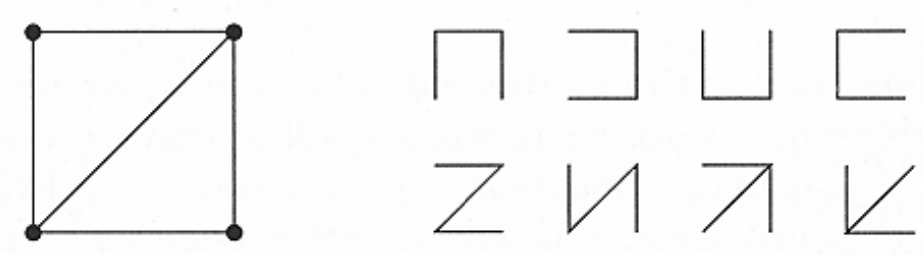
\includegraphics[width=.7\textwidth]{tree-spanning-tree}
  \caption{(2.2.6. Example in text) Three are 8 possible spanning trees (on the right) of a kite (on the left).}
  \label{fig:tree-spanning-tree}
\end{figure}

\begin{definition}{}{tree-contraction}
  (2.2.7. Definition in text)
  In a graph $G$, \textbf{contraction} of edge $e$ with endpoints $u,\, v$ is the replacement of $u$ and $v$ with a single vertex whose incident edges are the edges other than $e$ that were incident to $u$ or $v$. The resulting graph $G \cdot e$ has one less edge than $G$.
\end{definition}

\begin{figure}[htbp]
  % TODO: TikZ version
  \centering
  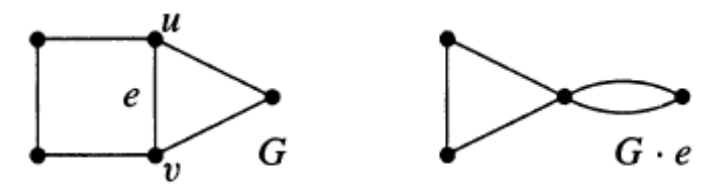
\includegraphics[width=.7\textwidth]{tree-contraction}
  \caption{A contraction of edge $e$ in graph $G$ on the left, is $G \cdot e$ on the right.}
  \label{fig:tree-contraction}
\end{figure}

In \cref{def:tree-contraction}, contraction is like compression. In a drawing of $G$, contraction of $e$ shrinks the edge to a single point. Contracting an edge can produce multiple edges or loops, but we leave them as they are. To count spanning trees correctly, we must keep multiple edges (see \cref{ex:tree-recursive-spanning-tree-count}). In other applications of contraction, the multiple edges may be irrelevant.

\begin{proposition}{}{tree-recursive-spanning-tree-count}
  (2.2.8. Proposition in text)
  Let $\tau(G)$ denote the number of spanning trees of a graph $G$.
  If $e \in E(G)$ is not a loop, then $\tau (G) = \tau (G - e) + \tau (G \cdot e)$.
\end{proposition}

\Cref{prop:tree-recursive-spanning-tree-count} is like a recursive relationship. We calculate the number of spanning trees of $G$ with the spanning tree counts of its subgraph and contraction recursively to divide and conquer the problem. Note that this proposition is not for the enumeration of spanning trees, but the count.

Note that $G \cdot e$ and $G$ are a bijection. To show the correctness of \cref{prop:tree-recursive-spanning-tree-count} with an example, in \cref{fig:tree-spanning-tree}, let the diagonal edge be $e$. There are two kinds of spanning tree of $G$. One is those with $e$, and the other is those without $e$ (as subgraphs of $G - e$). The spanning trees in $G \cdot e$ have one-to-one correspondence to the spanning trees that contain $e$ in $G$. So, we can calculate $\tau (G)$ with $\tau (G - e) + \tau (G \cdot e)$.

\begin{supplement}
  \textbf{Proof} of \cref{prop:tree-recursive-spanning-tree-count}:
  \begin{enumerate*}
    \item The spanning trees of $G$ that omit $e$ are precisely the spanning trees of $G - e$ (as a bijection).
    \item To show that $G$ has $\tau(G \cdot e)$ spanning trees containing $e$, we show that contraction of $e$ defines a bijection from the set of spanning trees of $G$ containing $e$ to the set of spanning trees of $G \cdot e$.
    \item When we contract $e$ in a spanning tree that contains $e$, we obtain a spanning tree of $G \cdot e$, because the resulting subgraph of $G \cdot e$ is spanning and connected and has the right number of edges.
    \item The other edges maintain their identity under contraction, so no two trees are mapped to the same spanning tree of $G \cdot e$ by this operation.'
    \item Also, each spanning tree of $G \cdot e$ arises in this way, since expanding the new vertex back into $e$ yields a spanning tree of $G$. Since each spanning tree of $G \cdot e$ arises exactly once, the function is a bijection.
  \end{enumerate*}
\end{supplement}

\begin{example}{A step in the recurrence}{tree-recursive-spanning-tree-count}
  (2.2.9. Example in text)
  In \cref{fig:tree-recursive-spanning-tree-count}, each of the graphs on the right has four spanning trees, so \cref{prop:tree-recursive-spanning-tree-count} implies that the kite has eight spanning trees. Without the multiple edges, the computation would fail.
\end{example}

\begin{figure}[htbp]
  % TODO: TikZ version
  \centering
  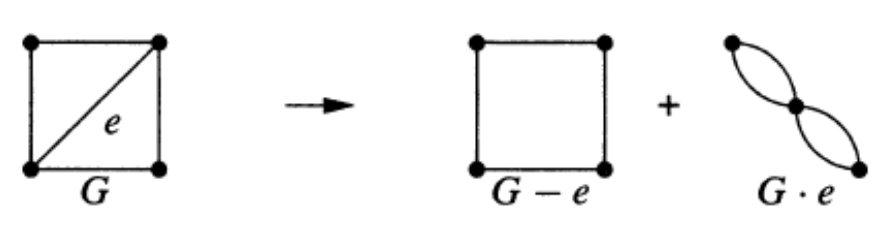
\includegraphics[width=.7\textwidth]{tree-recursive-spanning-tree-count}
  \caption{Graphs for \cref{ex:tree-recursive-spanning-tree-count}.}
  \label{fig:tree-recursive-spanning-tree-count}
\end{figure}

Note: We cannot apply the recurrence of \cref{prop:tree-recursive-spanning-tree-count} when $e$ is a loop. By definition, a self-loop is not a spanning tree. In some cases, you regard a self-loop as a spanning tree; if you utilize \cref{prop:tree-recursive-spanning-tree-count}, there will be two spanning trees as a wrong answer.

\begin{example}{A Matrix Tree computation}{tree-matrix-tree}
  To compute \cref{prop:tree-recursive-spanning-tree-count} by a program, we utilize the Matrix Tree computation.

  Let $Q$ be a matrix of a graph $G$. $Q_{ii}$ is the degree of vertex $i$. Let $a_{ij}$ be the number of edges between vertices $i$ and $j$ ($i \neq j$). $Q_{ij} = - a_{ij}$ ($i \neq j$). If there is no edge between vertices $i$ and $j$ ($i \neq j$), then $a_{ij} = 0$.

  Later, by utilizing \cref{thm:tree-matrix-tree}, we can calculate $\tau (G)$ by $Q$.

  \centering
  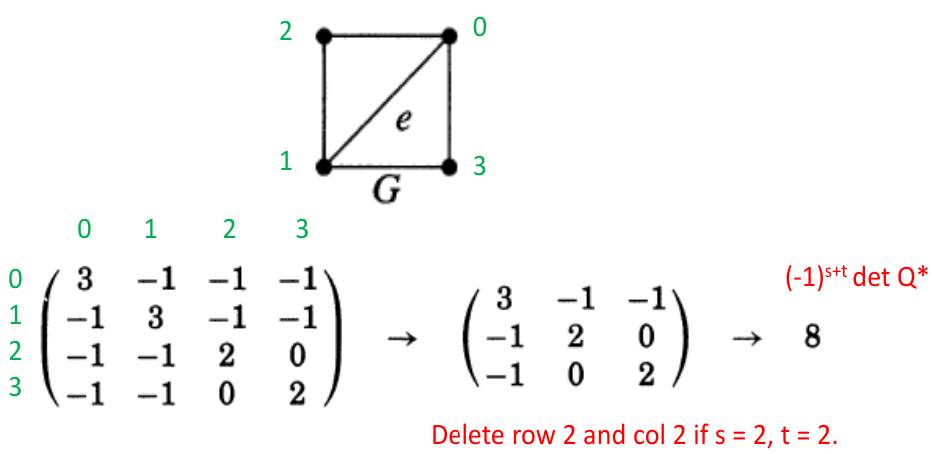
\includegraphics[width=.5\textwidth]{tree-matrix-tree}
\end{example}

\begin{theorem}{Matrix Tree Theorem}{tree-matrix-tree}
  (2.2.12. Theorem in text) Given a loopless graph $G$ with vertex set $v_1,\, \ldots,\, v_n$, let $a_{i, j}$ be the number of edges with endpoints $v_i$ and $v_j$. Let $Q$ be the matrix in which entry $(i, j)$ is $- a_{i, j}$ when $i \neq j$ and is $d \left( v_i \right)$ when $i = j$. If $Q^*$ is a matrix obtained by deleting row $s$ and column $t$ of $Q$, then $\tau (G) = (-1)^{s + t} \operatorname{det} Q^*$.
\end{theorem}

In \cref{thm:tree-matrix-tree}, $\operatorname{det} A = \abs{A}$ is the determinant of the matrix $A$.

\begin{definition}{}{tree-graceful}
  (2.2.14. Definition). A graceful labeling of a graph $G$ with $m$ edges is a function $f: V(G) \rightarrow \{0,\, \ldots,\, m\}$ such that distinct vertices receive distinct numbers and $\{\abs{f(u) - f(v)}: u v \in E(G)\} = \{1,\, \ldots,\, m\}$ (each edge is \textbf{uniquely} identified by the absolute difference between its endpoint indices). A graph is graceful if it has a graceful labeling.
\end{definition}

\begin{theorem}{}{tree-graceful-decomposition}
  (2.2.16. Theorem in text) (Rosa [1967]) If a tree $T$ with $m$ edges has a graceful labeling, then $K_{2 m + 1}$ has a decomposition into $2 m + 1$ copies of $T$.
\end{theorem}

In \cref{fig:tree-graceful}, the graph $G$ on the left with 4 edges is graceful. On the right, we have a $K_9$. By rotating $G$ 9 times, we can show \cref{thm:tree-graceful-decomposition}. The first one is the one with bold lines, and the second one is solid, and so on.

\begin{figure}[htbp]
  \centering
  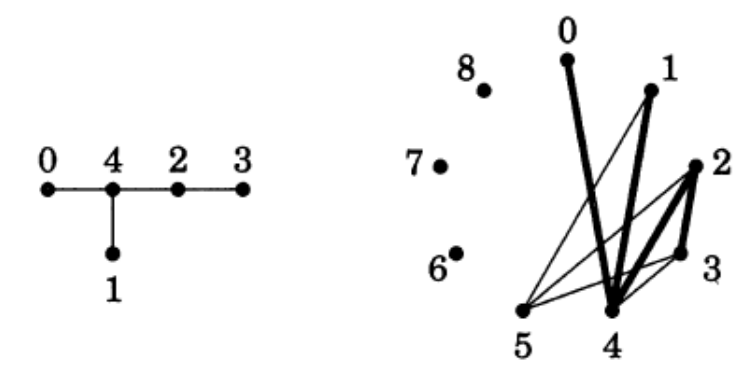
\includegraphics[width=.7\textwidth]{tree-graceful}
  \caption{An example of a graceful tree defined by \cref{def:tree-graceful}}
  \label{fig:tree-graceful}
\end{figure}

Direct \textbf{proof} of \cref{thm:tree-graceful-decomposition}:
\begin{enumerate*}
  \item View the vertices of $K_{2 m+1}$ as the congruence classes modulo $2 m + 1$, arranged circularly. The difference between two congruence classes is 1 if they are consecutive, 2 if one class is between them, and so on up to difference $m$. We group the edges of $K_{2 m + 1}$ by the difference between the endpoints. For $1 \leq j \leq m$, there are $2 m + 1$ edges with difference $j$.
  \item From a graceful labeling of $T$, we define copies of $T$ in $K_{2 m+1}$; the copies are $T_0, \ldots, T_{2 m}$. The vertices of $T_k$ are $k, \ldots, k+m(\bmod 2 m+1)$, with $k+i$ adjacent to $k+j$ if and only if $i$ is adjacent to $j$ in the graceful labeling of $T$. The copy $T_0$ looks just like the graceful labeling and has one edge with each difference. Moving to the next copy shifts each edge to another having the same difference by adding one to the name of each endpoint. Each difference class of edges has one edge in each $T_k$, and thus $T_0, \ldots, T_{2 m}$ decompose $K_{2 m+1}$.
\end{enumerate*}

\begin{definition}{}{tree-caterpillar}
  (2.2.17. Definition in text)
  A \textbf{caterpillar} is a tree in which a single path (the \textbf{spine}) is incident to (or contains) every edge.
\end{definition}

\begin{figure}[htbp]
  \centering
  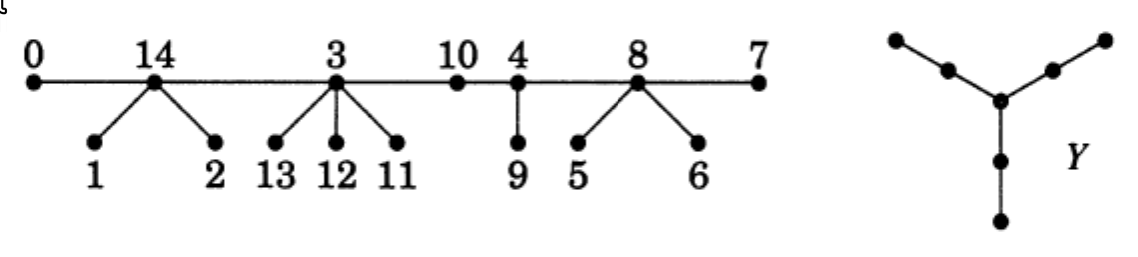
\includegraphics[width=.8\textwidth]{tree-caterpillar}
  \caption{The 0,7-path is the spine of the graph on the left because all the edges other than those on the 0,7-path are connected to the 0,7-path. The graph on the right (a Y graph) is not a caterpillar.}
  \label{fig:tree-caterpillar}
\end{figure}

\textbf{Bonus}: Prove that a caterpillar is graceful. (1 point)

\begin{theorem}{}{tree-caterpillar-from-tree}
  (2.2.19. Theorem in text)
  A tree is a caterpillar if and only if it does not contain the tree $Y$ above.
\end{theorem}

\textbf{Proof} of \cref{thm:tree-caterpillar-from-tree}: Let $G'$ denote the tree obtained from a tree $G$ by deleting each leaf of $G$. (For example, after deleting all leaves of $Y$, the center vertex with its neighbors must survive.) Since all vertices that survive in $G'$ are non-leaves in $G, G'$ has a vertex of degree at least 3 if and only if $Y$ appears in $G$. Hence $G$ has no copy of $Y$ if and only if $\Delta \left( G' \right) \leq 2$ ($\Delta \left( G' \right)$ is the maximum degree in $G'$; see \cref{def:con-degree}). This is equivalent to $G'$ being a path, which is equivalent to $G$ being a caterpillar.


\subsection{Optimization and Trees}

In this subsection, we'll introduce the three techniques helpful in Electrical Engineering: minimum spanning tree (MST), shortest paths, and binary decision diagram (BDD).

\begin{supplement}
  For example, in finding the program architecture bug or implementing software verification, we want the bug is discoverable via the shortest path in a program execution tree.

  In an integrated circuit (IC) or automation control, there may be a potential defect with some combination of signal. By using a binary decision tree (BDT), we prevent building a large truth table for the input. By using a binary decision diagram (BDD), we save more spaces in hardware or memory.
\end{supplement}

\subsubsection{Minimum Sapnning Tree (MST)}

All the algorithms introduced in this section has their own limitations. There is no a monolithic algorithm suitable that can find a MST from all kinds of graphs.

\begin{algorithm}{Kruskal's Algorithm - for minimum spanning trees}{tree-mst-kruskal}
  (2.3.1. Algorithm in text) C.f. Exercise 2.3.10 (Prim's algorithm)

  \textbf{Input}: A weighted connected graph.

  \textbf{Idea}: Maintain an acyclic spanning subgraph $H$, enlarging it by edges with low weight to form a spanning tree. (A minimum spanning tree, MST, is a spanning tree with the minimum possible total edge weight.) Consider edges in non-decreasing order of weight, breaking ties arbitrarily. \supp{Although in the process, $H$ may be a forest, it will be a spanning tree at the end. In the meanwhile, Prim's algorithm gaurentees $H$ being a tree in the process.}

  \textbf{Initialization}: Set $E(H) = \emptyset$.

  \textbf{Iteration}: If the next cheapest edge joins two components of $H$, then include it; otherwise, discard it. Terminate when $H$ is connected.
\end{algorithm}

In the exams, you may be asked to answer the process of a specific MST algorithm given a graph.

\begin{figure}[htbp]
  \centering
  \begin{subfigure}[t]{.25\textwidth}
    \centering
    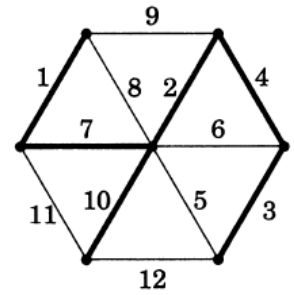
\includegraphics[width=.7\textwidth]{tree-mst-0}
    \caption{Initial graph}
    \label{fig:tree-mst-0}
  \end{subfigure}

  \begin{subfigure}[t]{.25\textwidth}
    \centering
    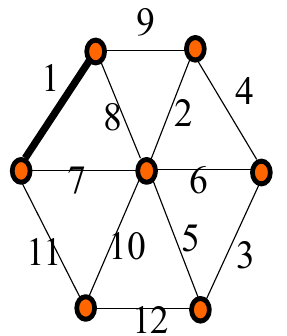
\includegraphics[width=.65\textwidth]{tree-mst-1}
    \caption{Step 1: Add the bold edge which has the minimum weight to the acyclic spanning subgraph $H$.}
    \label{fig:tree-mst-1}
  \end{subfigure}
  \hspace{.1\textwidth}
  \begin{subfigure}[t]{.25\textwidth}
    \centering
    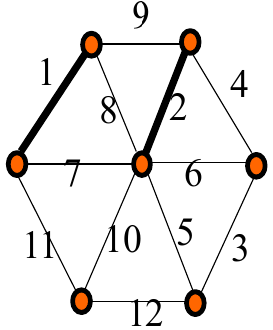
\includegraphics[width=.6\textwidth]{tree-mst-2}
    \caption{Step 2: Add 2, but form a forest.}
    \label{fig:tree-mst-2}
  \end{subfigure}
  \hspace{.1\textwidth}
  \begin{subfigure}[t]{.25\textwidth}
    \centering
    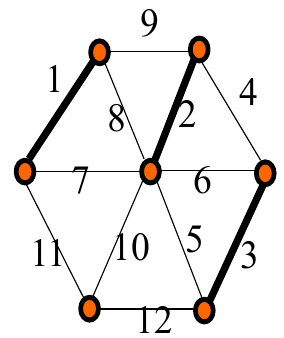
\includegraphics[width=.6\textwidth]{tree-mst-3}
    \caption{Step 3}
    \label{fig:tree-mst-3}
  \end{subfigure}

  \begin{subfigure}[t]{.25\textwidth}
    \centering
    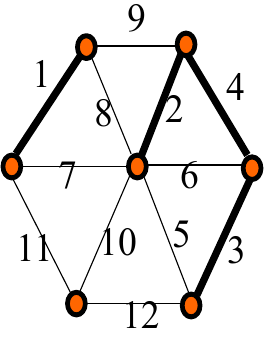
\includegraphics[width=.6\textwidth]{tree-mst-4}
    \caption{Step 4}
    \label{fig:tree-mst-4}
  \end{subfigure}
  \hspace{.1\textwidth}
  \begin{subfigure}[t]{.25\textwidth}
    \centering
    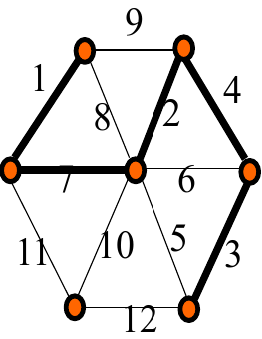
\includegraphics[width=.6\textwidth]{tree-mst-5}
    \caption{Step 5: Add 7 because adding 5 or 6 results in a cycle to break $H$.}
    \label{fig:tree-mst-5}
  \end{subfigure}
  \hspace{.1\textwidth}
  \begin{subfigure}[t]{.25\textwidth}
    \centering
    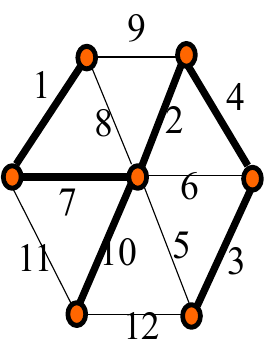
\includegraphics[width=.6\textwidth]{tree-mst-6}
    \caption{Step 6: Add 10 because we cannot add 5, 6, 8 or 9 without creating a cycle.}
    \label{fig:tree-mst-6}
  \end{subfigure}
  \caption{The process of Kruskal's algorithm.}
  \label{fig:tree-mst}
\end{figure}

\subsubsection{Shortest Paths}

Note that there may be multiple shortest paths, or there does not exist a shortest path for vertices between two components in a disconnected graph.

Shortest paths are defined on the paths with the lowest \textbf{weights} of edges instead of vertex or edge counts. For example, although a path via alleys is the shortest path, but a path via main roads requires the minimum time (weight).

\begin{algorithm}{Dijkstra's Algorithm--distances from one vertex}{tree-dijkstra}
  (2.3.5. Algorithm in text)

  \textbf{Input}: A graph (or digraph) with nonnegative edge weights and a starting vertex $u$. The weight of edge $x y$ is $w(x y)$; let $w(x y)=\infty$ if $x y$ is not an edge.

  \textbf{Idea}: Maintain the set $S$ of vertices to which a shortest path from $u$ is known, enlarging $S$ to include all vertices. To do this, maintain a tentative distance $t(z)$ from $u$ to each $z \notin S$, being the length of the shortest $u, z$-path yet found.

  \textbf{Initialization}: Set $S = \{ u \}$; $t(u) = 0$; $t(z) = w(u z)$ for $z \neq u$.

  \textbf{Iteration}: Select a vertex $v$ outside $S$ such that $t(v) = \min _{z \notin S} t(z)$. Add $v$ to $S$. Explore edges from $v$ to update tentative distances: for each edge $v z$ with $z \notin S$, update $t(z)$ to $\min \{ t(z),\, t(v) + w(v z)\}$.

  The iteration continues until $S = V(G)$ or until $t(z) = \infty$ for every $z \notin S$. At the end, set $d(u, v) = t(v)$ for all $v$.
\end{algorithm}

Time algorithm is useful in costs (like latencies) for a specific network topology, where the costs are nonnegative.

Note that finding shortest paths is an NP-complete problem, so Dijkstra's algorithm only provides a heuristic optimization for a special case (nonnegative edge weights).

For an unweighted graph or for a graph with identical edge weight, Dijkstra's algorithm acts like Breadth-First Search (BFS). C.f. BFS (2.3.8. Algorithm in text).

\begin{figure}[htbp]
  \centering
  \begin{subfigure}[t]{.45\textwidth}
    \centering
    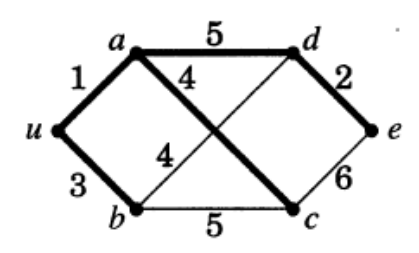
\includegraphics[width=.6\textwidth]{tree-dijkstra-0}
    \caption{Initial graph.}
    \label{fig:tree-dijkstra-0}
  \end{subfigure}
  \hfill
  \begin{subfigure}[t]{.45\textwidth}
    \centering
    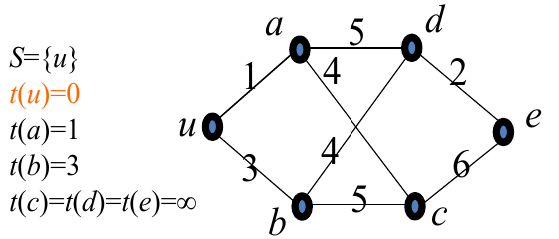
\includegraphics[width=.9\textwidth]{tree-dijkstra-1}
    \caption{Step 1: We visit $u$, so $S = \{ u \}$. The distance from $u$ to itself is 0 ($t(u) = 0$). Although there is a path from $u$ to $c,\, d,\, e$, but we see only vertices from $u$ now, so $t(c) = t(d) = t(e) = \infty$ now. The confirmed $t$ values are in orange.}
    \label{fig:tree-dijkstra-1}
  \end{subfigure}

  \begin{subfigure}[t]{.45\textwidth}
    \centering
    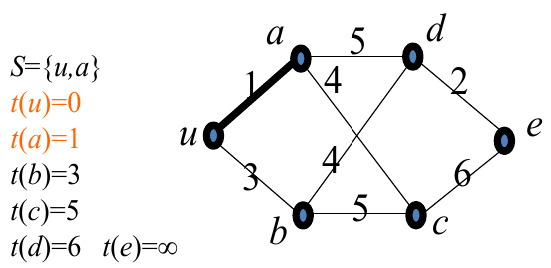
\includegraphics[width=.9\textwidth]{tree-dijkstra-2}
    \caption{Step 2: We visit $a$ because it is the nearest unconfirmed vertex from $u$ now.}
    \label{fig:tree-dijkstra-2}
  \end{subfigure}
  \hfill
  \begin{subfigure}[t]{.45\textwidth}
    \centering
    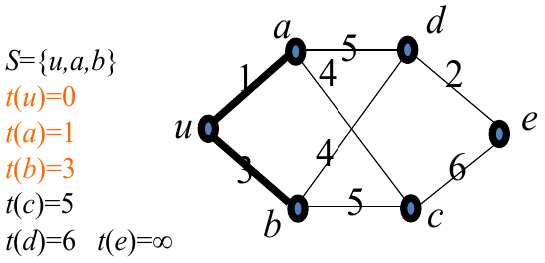
\includegraphics[width=.9\textwidth]{tree-dijkstra-3}
    \caption{Step 3}
    \label{fig:tree-dijkstra-3}
  \end{subfigure}

  \begin{subfigure}[t]{.45\textwidth}
    \centering
    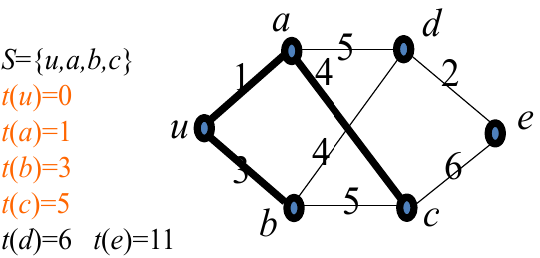
\includegraphics[width=.9\textwidth]{tree-dijkstra-4}
    \caption{Step 4}
    \label{fig:tree-dijkstra-4}
  \end{subfigure}
  \hfill
  \begin{subfigure}[t]{.45\textwidth}
    \centering
    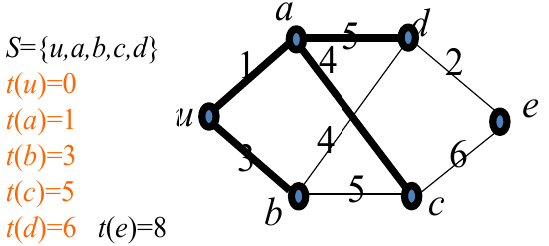
\includegraphics[width=.9\textwidth]{tree-dijkstra-5}
    \caption{Step 5}
    \label{fig:tree-dijkstra-5}
  \end{subfigure}

  \caption{The process of Dijkstra's algorithm on a sample connected graph.}
  \label{fig:tree-dijkstra}
\end{figure}

In exams, you may be asked to show the process of Dijkstra's algorithm step by step. Although some graph has an obvious solution, you need to show it step by step along with the updated values without haste.

\subsubsection{Binary Decision Diagram (BDD)}

Idea: By simplifying a diagram (graph), we can represent it with fewer nodes and edges.

\begin{enumerate}
  \item BDD is a data structure for switching functions that relies on a \textbf{compactification} (compression) of binary decision trees.
  \item The idea is to \textbf{skip redundant fragments} (duplicated subtrees or nodes) of a binary decision tree.
  \item Collapsing constant subtrees (i.e., subtrees where all terminal nodes have the same value) into a single node and identifying nodes with \textbf{isomorphic} subtrees.
  \item BDD is a \textbf{DAG} (directed acyclic graph) of outdegree 2:
    \begin{enumerate}
      \item Inner (internal) nodes are labeled by variables.
        \supp{For example, to represent gates of an IC in software, we use variables in boolean expressions.} We use a solid line for 1, and a dashed one for 0. \supp{However, using solid lines only with 0/1 labels on them is more clear and preferred by the instructor.}
      \item Outgoing edges are for possible evaluations of the corresponding variable.
      \item Terminal nodes are function values.
    \end{enumerate}
  \item With a \textbf{fixed variable ordering}, BDD can be a \textbf{minimal and canonical} (unique BDD for a function) form representation for Boolean formulae. Note that to have a \textbf{minimum} BDD, we need to try all variable orders. However, a relatively minimal BDD is enough for us.
\end{enumerate}

Isomorphic of graph $G$ and $H$ means a bijection (one-to-one and onto) between the sets of nodes of $G$ and $H$.

\begin{figure}[htbp]
  \centering
  \begin{subfigure}[t]{.3\textwidth}
    \centering
    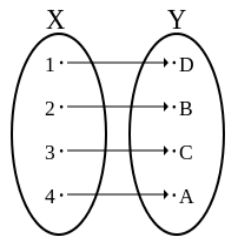
\includegraphics[width=.9\textwidth]{tree-bijection}
    \caption{Recall bijection (\cref{def:intro-bijection}).}
    \label{fig:tree-bijection}
  \end{subfigure}
  \hfill
  \begin{subfigure}[t]{.5\textwidth}
    \centering
    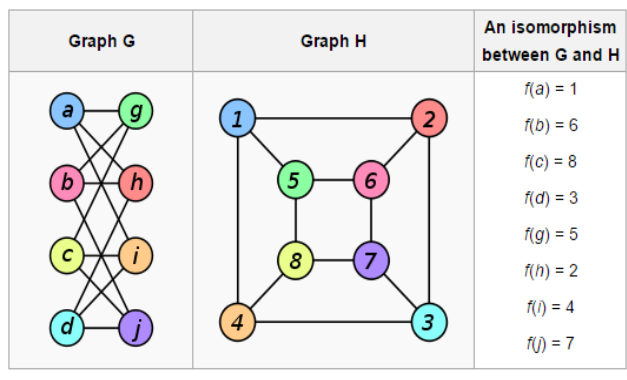
\includegraphics[width=.9\textwidth]{tree-isomorphism}
    \caption{Recall isomorphism (\cref{subsec:con-graph-isomorphism}).}
    \label{fig:tree-isomorphism}
  \end{subfigure}
  \caption{Recall bijection and isomorphism.}
  \label{fig:tree-bijection-isomorphism}
\end{figure}

Take $z_1 \land \left( \neg z_2 \lor z_3 \right)$ as example. See \cref{fig:tree-bdd}.

\begin{figure}[htbp]
  \centering
  \begin{subfigure}[t]{.6\textwidth}
    \centering
    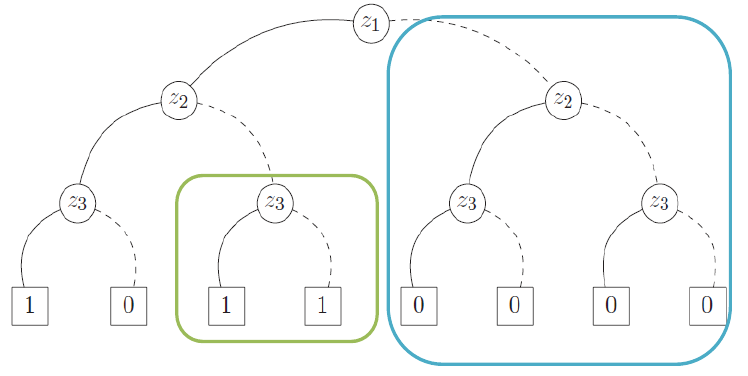
\includegraphics[width=.8\textwidth]{tree-bdd-0-bdt}
    \caption{You need 6 internal nodes and 14 edges to represent the binary decision tree.}
    \label{fig:tree-bdd-0-bdt}
  \end{subfigure}

  \begin{subfigure}[t]{.4\textwidth}
    \centering
    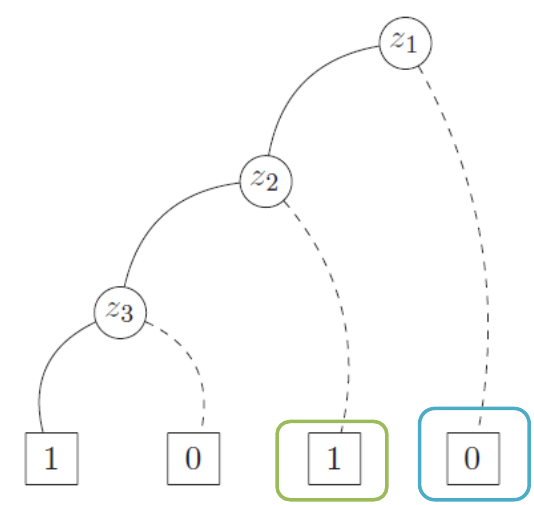
\includegraphics[width=.7\textwidth]{tree-bdd-1}
    \caption{Step 1: The right subtree of $z_1$ can be collapsed to 0, while the right subtree of $z_2$ is 1. This is a BDD but not minimal.}
    \label{fig:tree-bdd-1}
  \end{subfigure}
  \hfill
  \begin{subfigure}[t]{.4\textwidth}
    \centering
    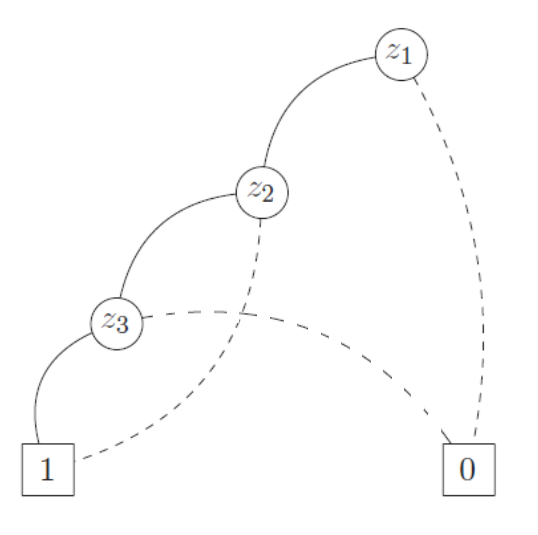
\includegraphics[width=.7\textwidth]{tree-bdd-2}
    \caption{Step 2: Combine shared leave nodes.}
    \label{fig:tree-bdd-2}
  \end{subfigure}

  \caption{An example of BDD for the boolean formulae $z_1 \land \left( \neg z_2 \lor z_3 \right)$.}
  \label{fig:tree-bdd}
\end{figure}

Exercise in class: Draw the following diagrams for $f=\left(z_1 \land z_3\right) \lor \left(z_2 \land z_3\right)$:
\begin{enumerate*}
  \item Binary Decision Tree
  \item Binary Decision Diagram
\end{enumerate*}



Before defining the ordered BDD, we need to define \textbf{variable ordering} in advance:
\begin{enumerate}
  % NOTE: \wp is the Weierstrass-p symbol, a weierstrass elliptic function, or
  % a uniquely fancy script p
  % ref: https://mathoverflow.net/a/278138
  % ref: https://mathoverflow.net/a/278932
  \item Let $Var$ be a finite set of variables. A \textbf{variable ordering} for Var denotes any tuple $\wp = \left(z_1, \ldots, z_m\right)$ such that $Var = \left\{z_1, \ldots, z_m \right\}$ and $z_i \neq z_j$ for $1 \leq i < j \leq m$. That is, variables are in a strictly increasing order.

  \item We write $<_{\wp}$ for the induced \textbf{total order} on $Var$. That is, for $\wp = \left( z_1,\, \ldots,\, z_m \right)$ the binary relation $<_{\wp}$ on $Var$ is given by $z_i <_{\wp} z_j$ if and only if $i < j$.

  \item We write $z_i \leqslant_{\wp} z_j$ iff. either $z_i <_{\wp} z_j$ or $i = j$.
\end{enumerate}

\textbf{$\bm{\wp}$-ordered binary decision diagram} ($\wp$-OBDD) is defined as:
\[\mathfrak{B} = \left( V,\, V_I,\, V_T,\, \successor_0,\, \successor_1,\, \var,\, \val,\, v_0 \right)\]
, where
\begin{enumerate*}
  \item $\mathfrak{B}$ is a fraktur $B$ symbol showing the \textbf{binary} property.
  \item $V$ is a finite set for nodes, and $V = V_I \cup V_T \cup v_0$.
  \item $V_I$ is the internal node set.
  \item $V_T$ is the terminal (leaf node) set.
  \item $v_0$ means the root of BDDs (boolean formula).
  \item $\successor_0$ and $\successor_1$ assign each inner node $v$ a 0-successor and 1-successor. $\successor_0(v) \in V$ and $\successor_1(v) \in V$. $\successor_0$ means the subtree that definitely evaluates to 0 in the BDT (tree). We don't say "subtree" because we focus on diagrams rather than trees.
\end{enumerate*}

$\wp$-OBDD:
\begin{enumerate}
  \item A variable labeling function $\var:\, V_I \rightarrow Var$ that assigns to each inner node $v$ a variable $\var(v) \in Var$.
  \item A value function $\val:\, V_T \rightarrow \{0,\, 1\}$ that assigns to each drain a function value 0 or 1.
  \item Consistency of the variable labeling function with the variable ordering $\wp$ is required in the following sense. If $\wp = \left( z_1,\, \ldots,\, z_m \right)$, then for each inner node $v$: if $\var(v) = z_i$ and $w \in \left\{ \successor_0(v), \successor_1(v)\right\} \cap V_I$, then $\var(w) = z_j$ for some $j > i$.
\end{enumerate}

\begin{figure}[htbp]
  \centering
  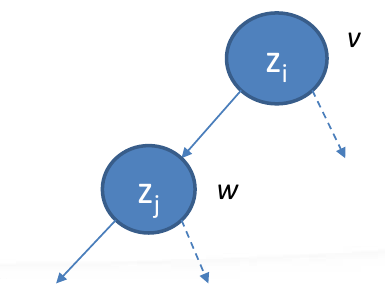
\includegraphics[width=.3\textwidth]{tree-obdd}
  \caption{Two internal nodes $v$ and $w$ in a $\wp$-OBDD, where the two nodes correspond to two boolean variables $z_i$ and $z_j$, respectively. \supp{If you need additional names for nodes, such names must be outside the nodes. However, we usually use the boolean variable names inside nodes without additional names.}}
  \label{fig:tree-obdd}
\end{figure}

\textbf{Minimality of Reduced OBDD} (ROBDD):

\begin{enumerate}
  \item When the variable ordering $\wp$ for $Var$ is fixed, then reduced $\wp$-OBDDs provide unique representations of switching functions for $Var$. (Of course, uniqueness is up to isomorphism)
  \item Two reduction rules for minimize $\wp$-OBDDs:
    \begin{enumerate}
      \item Elimination rule (\cref{fig:tree-robdd-elimination-rule}):

        If $v$ is an inner node of $\mathfrak{B}$ with $\successor_0(v) = \successor_1(v) = w$ ($v$ is not a determinant for results), then remove (eliminate) $v$ and redirect all incoming edges $u \rightarrow v$ to $w$.

      \item Isomorphism rule:

        It means if we have isomorphic structure in an OBDD, we can remove one copy or merge two copies into one.

        Specifically, if $v,\, w$ are nodes in $\mathfrak{B}$ with $v \neq w$ and either
        \vspace{1em}
        \begin{enumerate*}
          \item Case 1 (\cref{fig:tree-robdd-isomorphism-rule-1}): $v,\ w$ are drains with $\val(v) = \val(w)$
          \item Case 2 (\cref{fig:tree-robdd-isomorphism-rule-2}): $v, w$ are inner nodes with
            \vspace{-1em}
            $$
              \left\langle \var(v),\, \successor_1(v),\, \successor_0(v) \right\rangle =
              \left\langle \var(w),\, \successor_1(w),\, \successor_0(w) \right\rangle
            $$
        \end{enumerate*}
        , then remove node $v$ and redirect all incoming edges $u \rightarrow v$ to node $w$.
    \end{enumerate}
\end{enumerate}

\begin{figure}[htbp]
  \centering
  \begin{subfigure}[t]{.45\textwidth}
    \centering
    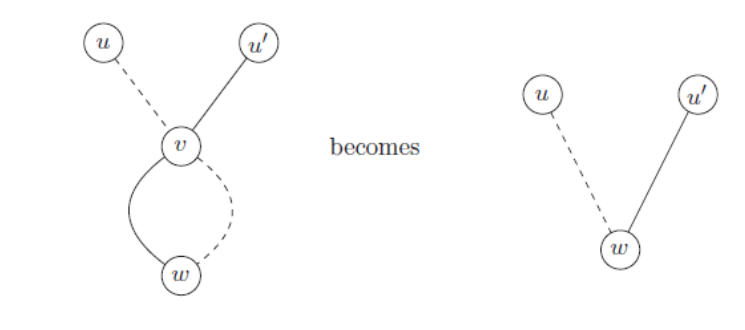
\includegraphics[width=\textwidth]{tree-robdd-elimination-rule}
    \caption{Elimination rule.}
    \label{fig:tree-robdd-elimination-rule}
  \end{subfigure}

  \begin{subfigure}[t]{.45\textwidth}
    \centering
    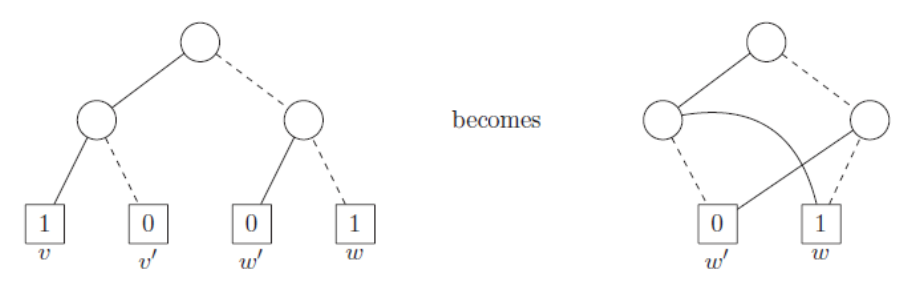
\includegraphics[width=\textwidth]{tree-robdd-isomorphism-rule-1}
    \caption{Isomorphism rule, case 1.}
    \label{fig:tree-robdd-isomorphism-rule-1}
  \end{subfigure}
  \hfill
  \begin{subfigure}[t]{.45\textwidth}
    \centering
    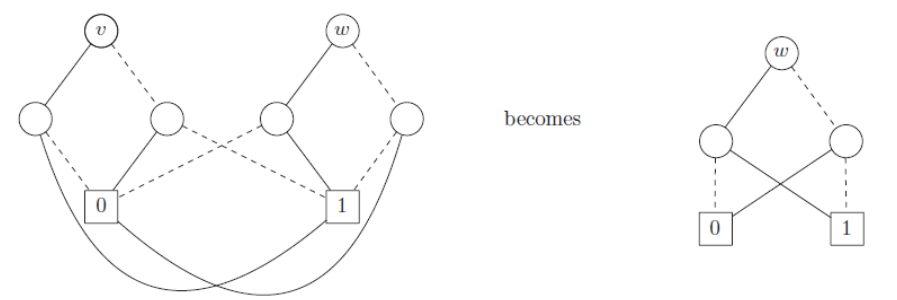
\includegraphics[width=\textwidth]{tree-robdd-isomorphism-rule-2}
    \caption{Isomorphism rule, case 2.}
    \label{fig:tree-robdd-isomorphism-rule-2}
  \end{subfigure}

  \caption{Examples of minimality of a reduced OBDD.}
  \label{fig:tree-robdd}
\end{figure}

\textbf{Shared OBDD} (SOBDD):
\begin{enumerate}
  \item Let $Var$ be a finite set of Boolean variables and $\wp$ a variable ordering for $Var$.
  \item A shared $\wp$-OBDD ($\wp$-SOBDD for short) is a tuple $\overline{\mathfrak{B}} = \left( V,\, V_I,\, V_T,\, \successor_0,\, \successor_1,\, \var,\, \val,\, \bar{v}_0 \right)$.
  \item The last component is a tuple $\bar{v}_0 = \left( v_0^1,\, \ldots,\, v_0^k \right)$ of roots.
  \item The requirements are as in $\wp$-ROBDDs, i.e., for all nodes $v,\, w \in V$
    \begin{enumerate*}
      \item $\var(v) <_{\wp} \var \left( \successor_b(v) \right)$ if $v \in V_I$ and $b \in\{0,1\}$, and
      \item $v \neq w$ implies $f_v \neq f_w$, where the switching function $f_v$ for the nodes $v \in V$ is defined as for OBDDs.
    \end{enumerate*}
\end{enumerate}

\begin{figure}[htbp]
  \centering
  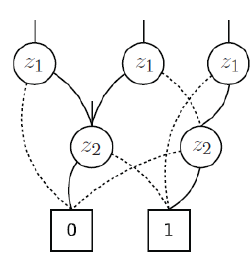
\includegraphics[width=.2\textwidth]{tree-sobdd}
  \caption{$z_1 \land \neg z_2$, $\neg z_2$, $z_1 \xor z_2$ and $\neg z_1 \lor z_2$ form a SOBDD with 4 root nodes (3 $z_1$ and the $z_2$ on the left with an arrow on its top).}
  \label{fig:tree-sobdd}
\end{figure}

\textbf{Boolean Operators}:
\begin{enumerate}
  \item \textbf{ITE operator}:

    ITE operator takes as arguments three switching functions $g,\, f_1,\, f_2$ and composes them according to "if $g$ then $f_1$ else $f_2$ ". Formally:
    \[
      \ite\left(g, f_1, f_2\right) =
      \left( g \land f_1 \right) \lor \left( \neg g \land f_2 \right)
    \]

    Special cases: $g$ is constant 0 or 1:
    \begin{align*}
      \ite\left( 0,\, f_1,\, f_2 \right) & = f_2 \\
      \ite\left( 1,\, f_1,\, f_2 \right) & = f_1
    \end{align*}

  \item Shannon Expansion:
    If $f$ is a switching function (0 or 1) for $Var$, then for each variable $z \in Var$:
    \[
      f =
      \left( \neg z \land \left. f \right|_{z = 0} \right) \lor
      \left( z \land \left. f \right|_{z = 1} \right)
    \]
    Rewritten with the ITE:
    \[
      f_v = \ite\left( z,\, f_{\successor_1(v)}, f_{\successor_0(v)} \right)
    \]

  \item Other Boolean operators by using ITE:
    \begin{align*}
      \neg f              & = \ite\left( f,\, 0,\, 1 \right)                             \\
      f_1 \vee f_2        & = \ite\left( f_1,\, 1,\, f_2 \right)                         \\
      f_1 \wedge f_2      & = \ite\left( f_1,\, f_2,\, 0 \right)                         \\
      f_1 \xor f_2        & = \ite\left( f_1,\, \neg f_2,\, f_2 \right)                  \\
      f_1 \xor f_2        & = \ite\left( f_1,\, \ite\left(f_2, 0,1\right),\, f_2 \right) \\
      f_1 \rightarrow f_2 & = \ite\left( f_1,\, f_2,\, 1 \right)
    \end{align*}
\end{enumerate}

\textbf{BDD operation}:
\begin{enumerate}
  \item Basic operator for efficient BDD structural manipulation:
    \begin{enumerate*}
      \item Based on recursive Shannon Expansion.
      \item Same semantics by using ITE.
    \end{enumerate*}

  \item Let $B_1$ and $B_2$ be two switching functions.
    \[
      B_1 \op B_2 =
      \left[ \neg \left( x_i \right) \left(\left. B_1 \right|_{x_i = 0} \op B_2 \right) \right] \lor
      \left[ \left( x_i \right) \left( \left. B_1 \right|_{x_i = 1} \op B_2 \right) \right]
    \]
    , where $\op$ can be OR, AND, XOR, $\ldots$, etc. See \cref{fig:tree-bdd-op} for the illustration.

  \item Case 1: $B_1$ and $B_2$ have the same root (saying $x_i$) as illustrated in \cref{fig:tree-bdd-op-same-root}.

  \item Case 2: $B_1$ and $B_2$ have different roots (saying $x_i$ and $x_k$) as illustrated in \cref{fig:tree-bdd-op-different-roots}:
    \begin{enumerate}
      \item Suppose the ordering is $x_i < x_k$, and we process $x_i$ first as illustrated \cref{fig:tree-bdd-op}.
      \item Then take $B_1^1$ and $B_1^0$ as two new $B_1$ to recursively construct the following trees (based on either case 1 or case 2), respectively.
    \end{enumerate}
\end{enumerate}

\begin{figure}[htbp]
  \centering
  \begin{subfigure}[t]{.45\textwidth}
    \centering
    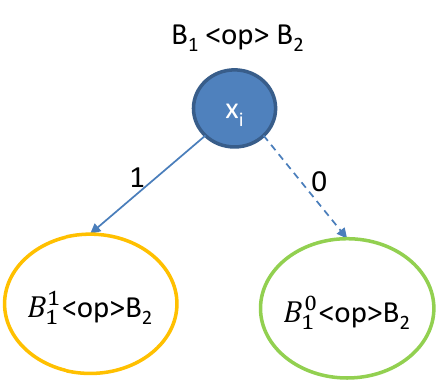
\includegraphics[width=.6\textwidth]{tree-bdd-op}
    \caption{$B_1 \op B_2$}
    \label{fig:tree-bdd-op}
  \end{subfigure}
  \hfill
  \begin{subfigure}[t]{.45\textwidth}
    \centering
    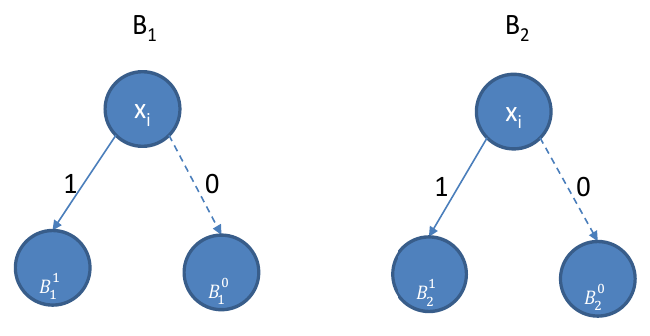
\includegraphics[width=\textwidth]{tree-bdd-op-same-root}
    \caption{$B_1 \op B_2$ with the same root ($x_1$)}
    \label{fig:tree-bdd-op-same-root}
  \end{subfigure}

  \begin{subfigure}[t]{.45\textwidth}
    \centering
    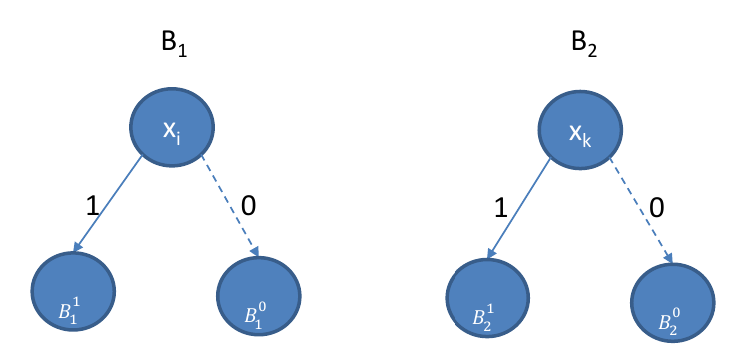
\includegraphics[width=\textwidth]{tree-bdd-op-different-roots}
    \caption{$B_1 \op B_2$ with different roots ($x_i$ and $x_k$).}
    \label{fig:tree-bdd-op-different-roots}
  \end{subfigure}
  \hfill
  \begin{subfigure}[t]{.5\textwidth}
    \centering
    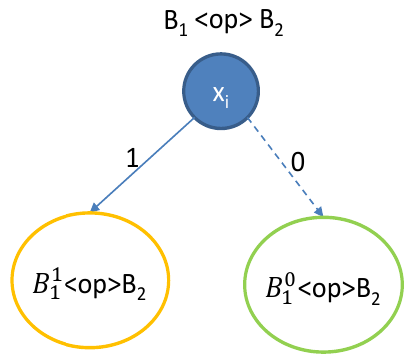
\includegraphics[width=.6\textwidth]{tree-bdd-op-different-roots-first}
    \caption{Process only $B_1$ rooted at $x_i$ from \cref{fig:tree-bdd-op-different-roots}. Note that $B_2$ comes without a superscript because we leave $B_2$ as it is now.}
    \label{fig:tree-bdd-op-different-roots-first}
  \end{subfigure}
  \caption{BDD operations.}
  \label{fig:tree-bdd-op-figures}
\end{figure}

In the exams, you may be given two Boolean formula $B_1$ and $B_2$, and you need to generate their own BDD. With the given operator, you need to perform the operation on the two BDDs.

\begin{example}{}{tree-bdd-op}
  \textbf{Question}: Let $B_1 = \neg \left( x_1 \lor x_3 \right)$, $B_2 = x_2 \land x_3$, and $\op$ is OR. (1) Please derive the BDDs of $B_1$ and $B_2$. (2) Please perform the operation $\op$. That is, $B_1 \lor B_2$.

  \textbf{Solution}: \cref{fig:tree-bdd-op-example}
\end{example}

\begin{figure}[htbp]
  \centering
  \begin{subfigure}[t]{.45\textwidth}
    \centering
    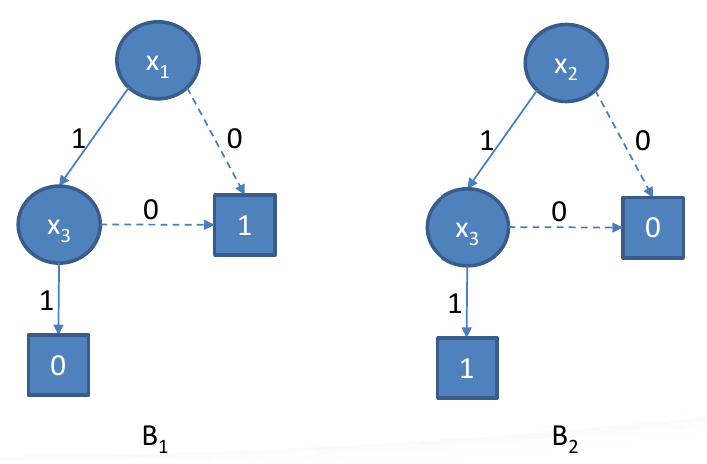
\includegraphics[width=.7\textwidth]{tree-bdd-example-step-0}
    \caption{Question part 1: Two BDDs.}
    \label{fig:tree-bdd-op-example-step-0}
  \end{subfigure}
  \hfill
  \begin{subfigure}[t]{.45\textwidth}
    \centering
    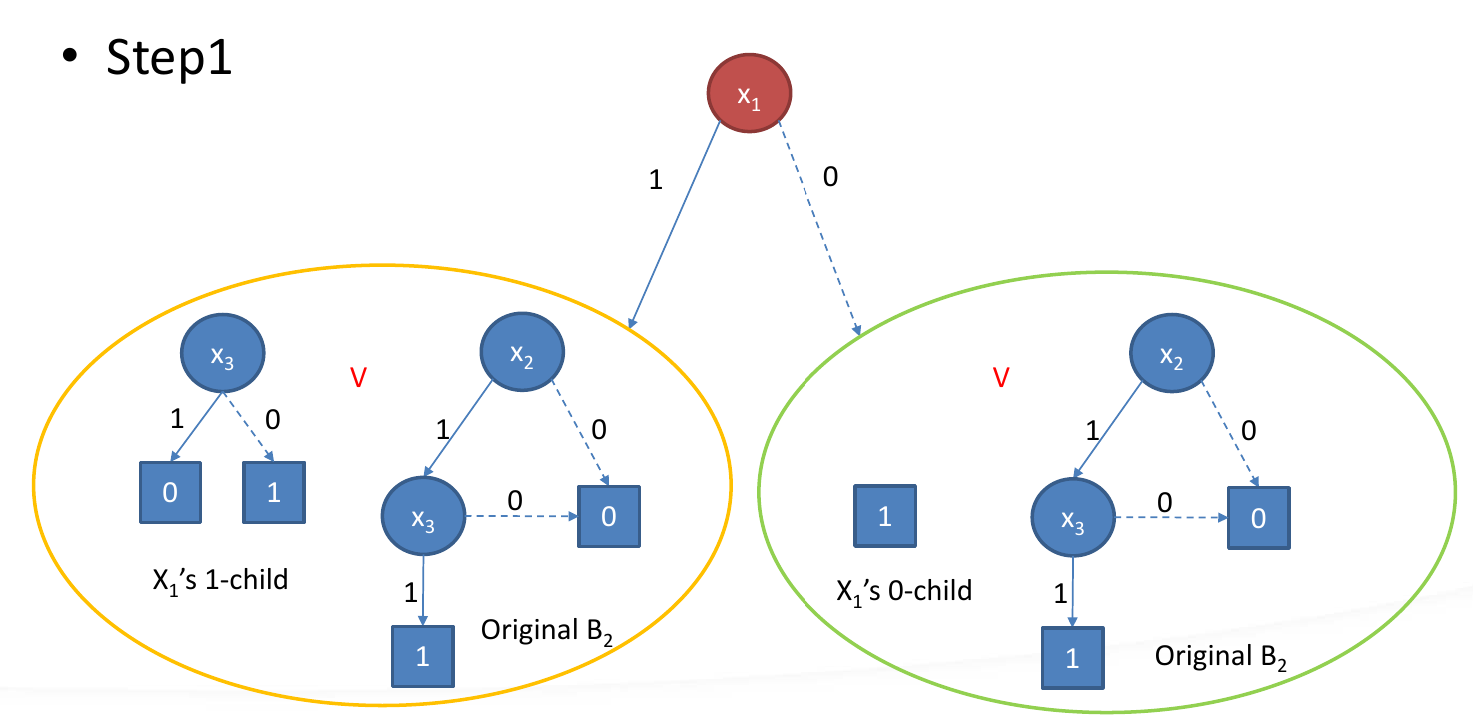
\includegraphics[width=\textwidth]{tree-bdd-example-step-1}
    \caption{Step 1: Let $x_1$ (vertex with the lowest index) be the root of the result BDD. 1-successor on the left contains $x_3$ along with its successors, and the entire $x_2$.}
    \label{fig:tree-bdd-op-example-step-1}
  \end{subfigure}

  \begin{subfigure}[t]{.45\textwidth}
    \centering
    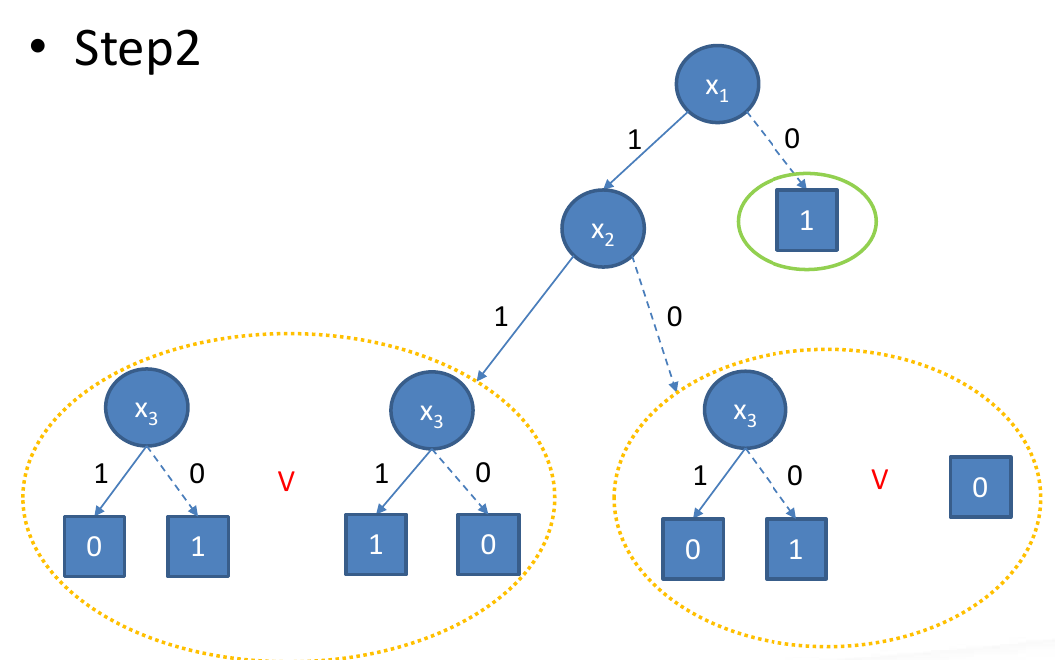
\includegraphics[width=\textwidth]{tree-bdd-example-step-2-1}
    \caption{Step 2-1: The red $V$ means the OR operator. 0-successor of $x_1$ evaluates to 1 because "1 OR anything" is 1.}
    \label{fig:tree-bdd-op-example-step-2-1}
  \end{subfigure}
  \hfill
  \begin{subfigure}[t]{.45\textwidth}
    \centering
    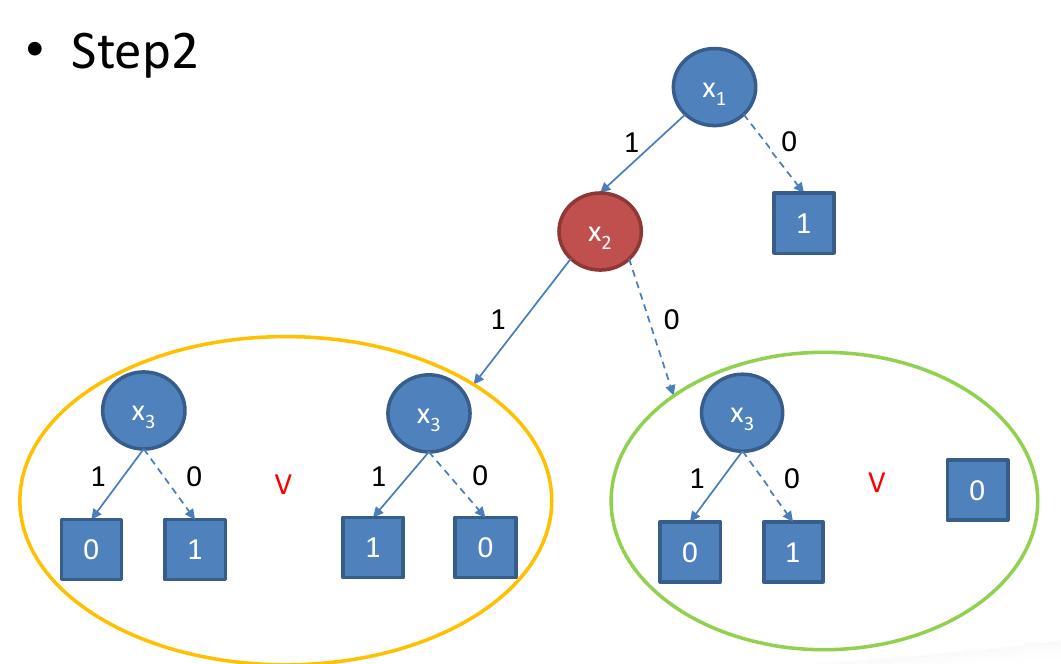
\includegraphics[width=\textwidth]{tree-bdd-example-step-2-2}
    \caption{Step 2-2: Take $x_2$ as the root of the 1-successor of $x_1$, and follow the process of different roots like step 1.}
    \label{fig:tree-bdd-op-example-step-2-2}
  \end{subfigure}

  \begin{subfigure}[t]{.45\textwidth}
    \centering
    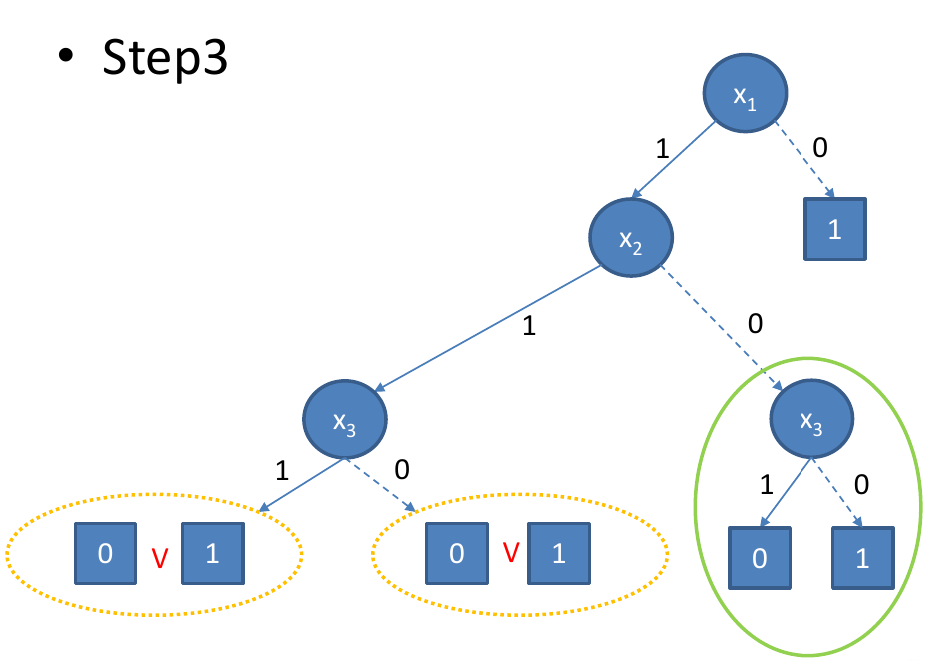
\includegraphics[width=.9\textwidth]{tree-bdd-example-step-3-1}
    \caption{Step 3-1: 0 in the 0-successor of $x_2$ is useless, so we remove it.}
    \label{fig:tree-bdd-op-example-step-3-1}
  \end{subfigure}
  \hfill
  \begin{subfigure}[t]{.45\textwidth}
    \centering
    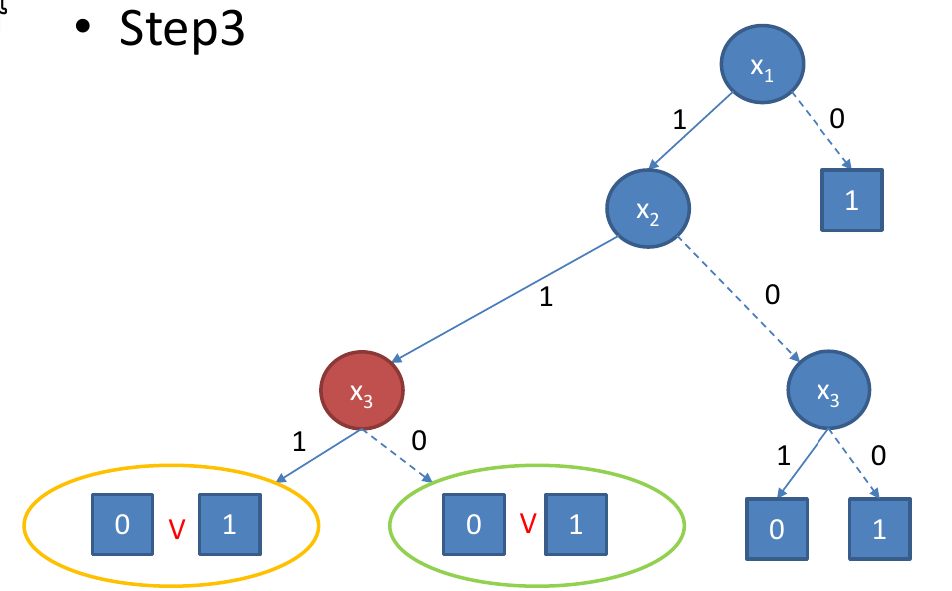
\includegraphics[width=.9\textwidth]{tree-bdd-example-step-3-2}
    \caption{Step 3-2: Take $x_3$ as the root of the 1-successor of $x_2$.}
    \label{fig:tree-bdd-op-example-step-3-2}
  \end{subfigure}

  \begin{subfigure}[t]{.3\textwidth}
    \centering
    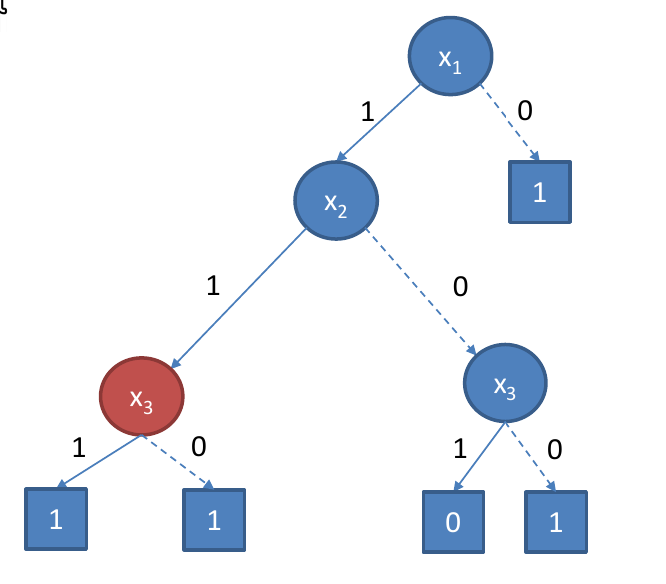
\includegraphics[width=.9\textwidth]{tree-bdd-example-step-3-3}
    \caption{Step 3-3: Evaluate the 1-successor and 0-successor of $x_3$ to 1 like step 2-1.}
    \label{fig:tree-bdd-op-example-step-3-3}
  \end{subfigure}
  \hspace{.025\textwidth}
  \begin{subfigure}[t]{.3\textwidth}
    \centering
    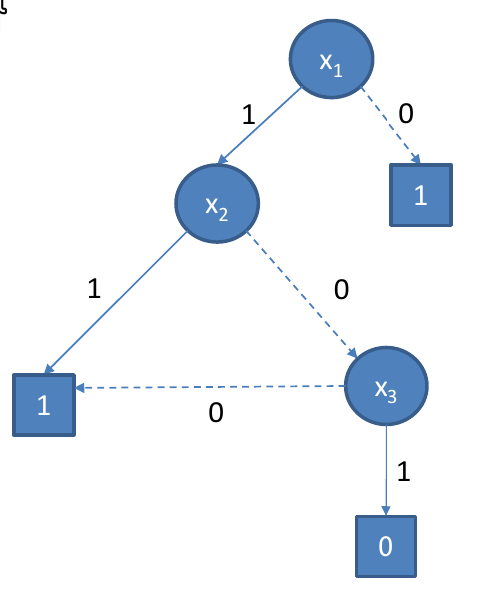
\includegraphics[width=.7\textwidth]{tree-bdd-example-step-4-1}
    \caption{Step 4-1: Retain a single $x_3$.}
    \label{fig:tree-bdd-op-example-step-4-1}
  \end{subfigure}
  \hspace{.025\textwidth}
  \begin{subfigure}[t]{.3\textwidth}
    \centering
    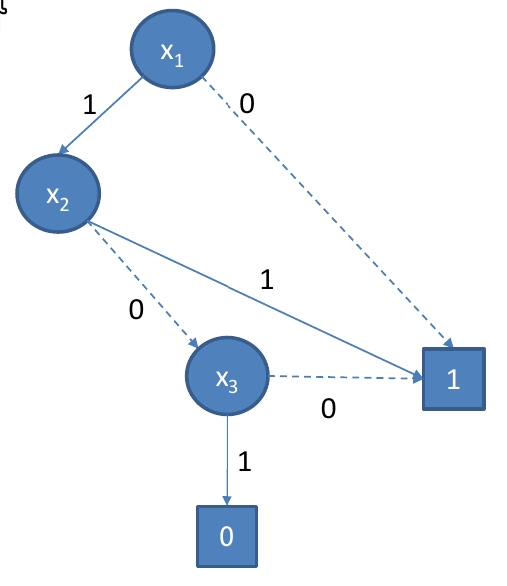
\includegraphics[width=.7\textwidth]{tree-bdd-example-step-4-2}
    \caption{Step 4-2: Redirect 1 leaves to a single 1. This is the final result.}
    \label{fig:tree-bdd-op-example-step-4-2}
  \end{subfigure}

  \caption{Solution to \cref{ex:tree-bdd-op}}
  \label{fig:tree-bdd-op-example}
\end{figure}

\end{document}